%%
%% This is file `thesis-test.tex',
%% generated with the docstrip utility.
%%
%% The original source files were:
%%
%% nuthesis.dtx  (with options: `thesis-test')
%% 

\documentclass[ms]{nuthesis}
%% Needed to typset the math in this sample
\usepackage{amsmath}
\usepackage{amsfonts}
%% Let's use a different font
\usepackage[sc,osf]{mathpazo}

%% prevents placing floats before a section
\usepackage[section]{placeins}

%% Makes things look better
\usepackage{microtype}

%% Makes things look better
\usepackage{booktabs}

%% Gives us extra list environments
\usepackage{paralist}

%% Be able to include graphicsx
\usepackage{graphicx}

%% Be able to use subfigure
\usepackage{caption}
\usepackage{subcaption}

%% I like darker colors
\usepackage{color}
\definecolor{dark-red}{rgb}{0.6,0,0}
\definecolor{dark-green}{rgb}{0,0.6,0}
\definecolor{dark-blue}{rgb}{0,0,0.6}

%% If you use hyperref, you need to load memhfixc *after* it.
%% See the memoir docs for details.
\usepackage[%
pdfauthor={James D. Duin},
pdftitle={Hierachical Active Learning Bioinformatics Application},
pdfsubject={BioDataset},
pdfkeywords={semi-supervised learning, active learning, hierarchical labeling, cost analysis},
linkcolor=dark-blue,
pagecolor=dark-green,
citecolor=dark-blue,
urlcolor=dark-red,
%colorlinks=true,
backref,
plainpages=false,% This helps to fix the issue with hyperref with page numbering
pdfpagelabels% This helps to fix the issue with hyperref with page numbering
]{hyperref}

%% Needed by memoir to fix things with hyperref
\usepackage{memhfixc}
\begin{document}
%% Start formating the first few special pages
%% frontmatter is needed to set the page numbering correctly
\frontmatter

\title{Hierachical Active Learning Bioinformatics Application}
\author{James D. Duin}
\adviser{Professor Stephen Scott}
\adviserAbstract{Stephen Scott}
\major{Computer Science}
\degreemonth{February}
\degreeyear{2017}
%%
%% For most people the defaults will be correct, so they are commented
%% out. To manually set these, just uncomment and make the needed
%% changes.
%% \college{Your college}
%% \city{Your City}
%%
%% For most people the following can be changed with a class
%% option. To manually set these, just uncomment the following and
%% make the needed changes.
%% \doctype{Thesis or Dissertation}
%% \degree{Your degree}
%% \degreeabbreviation{Your degree abbr.}
%%
%% Now that we know everything we need, we can generate the title page
%% itself.
%%
\maketitle
%% You have a maximum of 350, which includes your title, name, etc.
\begin{abstract}
  \par I made the classifiers to predict the BioDataset, I made the
  plots for the Active Passive curves, I made the plots for the Fixed
  Fine Ratio experiments with various costs.
\end{abstract}

%% Optional
%\begin{copyrightpage}
%This file may be distributed and/or modified under the conditions of
%the \LaTeX{} Project Public License, either version 1.3c of this license
%or (at your option) any later version.  The latest version of this
%license is in:
%\begin{center}
%   \url{http://www.latex-project.org/lppl.txt}
%\end{center}
%and version 1.3c or later is part of all distributions of \LaTeX version
%2006/05/20 or later.
%\end{copyrightpage}

%% Optional
\begin{dedication}
  This thesis is dedicated to my parents Paul and Vicki Duin and fiancee Anna Spady.
\end{dedication}

%% Optional
\begin{acknowledgments}
  I would like to thank my advisor Dr. Stephen Scott for guidance in selecting this
  research topic, Yugi Mo for his work in developing the HAL methodology, and Dr.
  Douglas Downey for his work on this topic. I would like to thank Juan Cui, Jiang Shu,
  Kevin Chiang for assistance accessing and understanding the protein dataset that is
  the subject of the paper.
\end{acknowledgments}

%% Optional
%\begin{grantinfo}
%  I'm not funded by any grants.
%\end{grantinfo}
%%% The ToC is required
%%% Uncomment these if need be

%% The ToC is required
\tableofcontents
%% Uncomment these if need be
%\listoffigures
%\listoftables

%%   mainmatter is needed after the ToC, (LoF, and LoT) to set the
%%   page numbering correctly for the main body
\mainmatter

%% Thesis goes here
\chapter{Introduction}\label{chap:aenied}
\section{Machine Learning}
\par Machine Learning algorithms are defined as computer programs that learn from experience E
with respect to some class of tasks T and performance measure P, if their performance at
tasks in T, as measured by P, improves with experience E [4]. In the context of this paper,
the machine learning algorithm that is used is a support vector machine (SVM) implementation
by libSvm [3]. The performance measure is the classification of protein instances according to a
label, for example, originated in the mitochondria or not.  The experience is the number of
training instances in the training set. The dataset is initially partitioned into training
and test sets. The algorithm improves its classifier structure based on the features of
each instance by iterating through all instances in the training set. When training has
been completed, the classifier is then tested on the test set and the number of instances
that the classifier correctly or incorrectly labels determines its accuracy, precision
and recall scores. In our protein dataset there are 20,098 proteins with 449 features each
relating to their structure. In our experiments an SVM classifier is applied to the dataset
with the goal of achieving high precision scores for the label “mitochondrion”, that is,
if the protein originates in the mitochondria or not.


\section{Hierarchical Bioinformatics Data Set}
\par The protein dataset is labeled according to where it originates in the cell.
At the root is “mitochondrion”, then there is the sub level labels for if its native
to the mitochondria or if it has a separate target compartment specification. The complete
tree along with the number of instances belonging to the each label is included in \textit{Figure} \ref{fig:Mito_tree}.

\FloatBarrier
\begin{figure}[!htb]
	\centering
    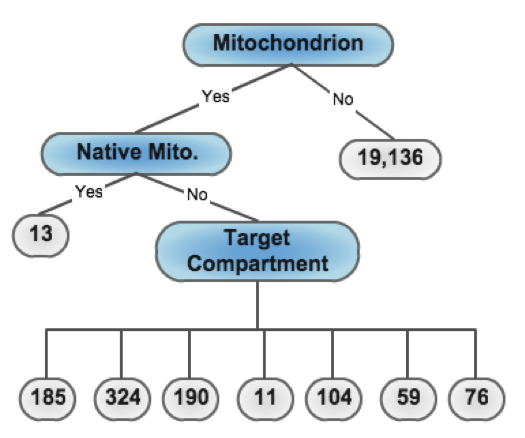
\includegraphics[width=0.5\columnwidth]{fig/Mito_tree}
    \label{fig:Mito_tree}
    \caption{The protein dataset is labeled according to where it originates in the cell. At the
    root is “mitochondrion”, then there is the sub level labels for if its native to the mitochondria
    or if it has a separate target compartment specification. The complete tree along with the number
    of instances belonging to the each label is included in \ref{fig:Mito_tree}.}
\end{figure}
\FloatBarrier

\section{Coarse Grained vs Fine Grained Trade Off}
\par The classifier that does not take advantage of any of the fine grained labels works off of the root
labels for each instance and does not train separate classifiers for the fine grained labels. This
classifier is referred to as the coarse grained classifier. The classifier that does use fine grained
labels, and trains a separate classifier for each label, then combines them to generate a root level
label is referred to as the fine grained classifier. It can be demonstrated through a dummy example
that for certain datasets, a fine grained approach to the root level classifier can achieve higher
levels of precision for the same level of recall. Such a dataset is shown in \ref{fig:union}. The
classifiers for this dataset can be thought of as a function of axis parallel rectangular boxes.
For the course grained to have high recall and return all of the positive circle instances, it must
encompass the entire dataset and incidentally return all of the negative diamond instances as
positive also. A fine grained approach is preferable for the dummy dataset pictured. It is the
intention of this study to demonstrate that the fine grained classification approach for a root
level classifier will achieve higher levels of precision for the same level of recall when
applied to the protein dataset.

\FloatBarrier
\begin{figure}[!htb]
	\centering
    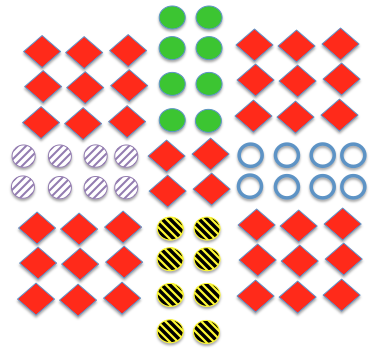
\includegraphics[width=0.5\columnwidth]{fig/union}
    \label{fig:union}
    \caption{Demonstration of a dataset that would benefit from multiple fine grained
    learners for each circle type. In order for the coarse grain learner to have high
    recall, precision must be scarified and a large amount of false positives returned.
    By combining fine grained classifiers the same level of recall can be achieved with a
    higher level of precision because none of the false positive diamonds will be returned}
\end{figure}
\FloatBarrier


\chapter{Background and Related Work}
\section{Active Learning}
\par Active Learning relates to the coarse grained vs fine grained tradeoff because it is
reasonable to assume that fine grained labels may not be as readily available as coarse grained
labels, and thus have a higher cost. An active learning approach is used to determine how
many fine grained labels to purchase in order to minimize the total cost to train the
algorithm an maximize the precision and recall scores. The following equations for
precision, recall, and a weighted F score are shown below in equations 1 through 3.
\break
$Precision eqn$ \break
$Recall eqn$ \break
$F0_5 eqn$ \break
\break
\par The goal in an active learning approach is to maximize the F measure where β equals 0.5 [2].
The F-0.5 measure gives more weight to precision, as opposed to recall, so it gives
incentive to purchase enough fine grained labels to increase the F-0.5 measure. The
coarse grained labels will cost less than fine grained labels, but the increase in
the F-0.5 measure justifies the increase in cost up to a certain point. The F-0.5
measure is used in the results section of this paper. ... That's why we use PRauc in the results.

\section{Other Papers cited by Yugi}
Describe some of the other papers that Yugi cited.

\section{Hierarchical Active Learning}
\par The Hierarchical Active Learning algorithm (HAL) is shown diagrammatically in Figure 3.
Multiple fine grained classifiers are trained at each level of the Hierarchy of the dataset.
Queries to the oracle are performed purchase the most cost effective labels to add to the
training sets of the classifiers. The active learning cycle continues until a cost budget has
been reached. The benefit of an active learning approach is to maximize the F-0.5 measure
for a given cost budget. It was the goal of this study to apply the HAL algorithm to the
protein dataset, however this is not achieved at this time. An existing application of
HAL is briefly discussed in the following section.


\FloatBarrier
\begin{figure}[!htb]
	\centering
    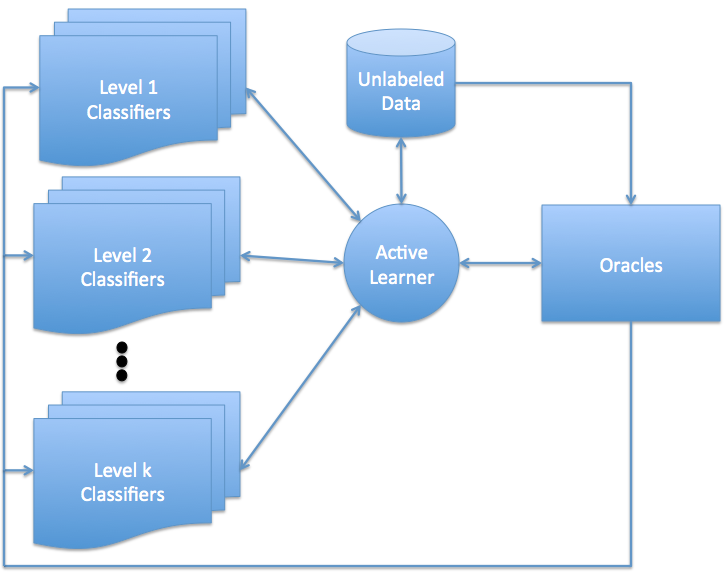
\includegraphics[width=0.5\columnwidth]{fig/AL2}
    \label{fig:AL2}
    \caption{Diagram of HAL approach}
\end{figure}
\FloatBarrier



\section{Application to Dispatch Dataset}
\par HAL was applied to a Dispatch dataset. This dataset contains 375,026 manually labeled
hierarchical names across 1,384 newspaper articles [2]. This is a clear example where
fine grained labels have a higher cost since it is easier for a person to manually
determine if the article pertains to an organization or not, rather than if it pertains
to a railroad or a zoo, which would be sub labels of the organization root. The first
analysis step was to determine that the F-0.5 measure is increased by using fine
grained classifiers. The results are shown in Figure 4. The highest F-0.5 measure for
a given iteration of purchases of training instances is obtained by using the active
learning approach with all fine-grained labels. The passive learning curves were
 generated by selecting batches of instances randomly rather than querying the
 oracle for a specific label type that offers that most gain in classifier accuracy.
 The active learning curves did take advantage of querying for specific labels in
 order to maximize gain in classifier accuracy. ... add other data sets.

\FloatBarrier
\begin{figure}[!htb]
	\centering
    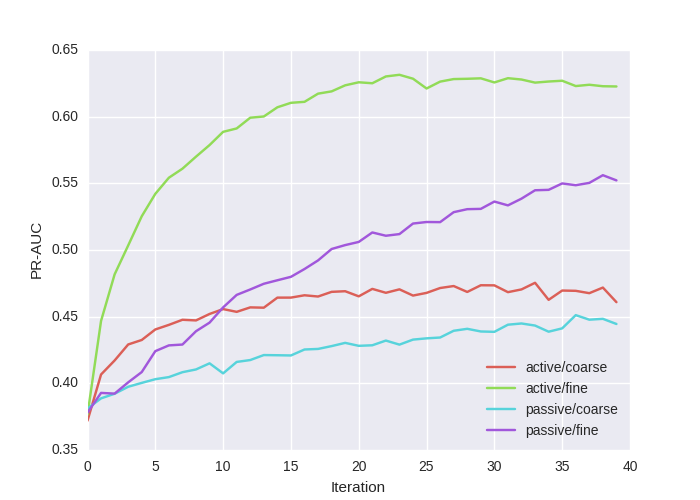
\includegraphics[width=1.0\columnwidth]{fig/draft-richmond}
    \label{fig:draft-richmond}
    \caption{Application of HAL demonstrating the benefit of Actively selecting the type
    of labels to purchase for instances rather than randomly selecting labels to purchase,
    as in the Passive curves.}
\end{figure}
\FloatBarrier


\par The next analysis step is to apply a given ratio of fine grained vs coarse grained
labels to purchase at each batch request to the oracle. The results of varying the
percentage of fine grained labels purchased are shown in Figure 5. The figure shows
that even a small amount of fine grained labels purchased, that is, 20perc provides a
significant increase in the F-0.5 measure for a given iteration. ...  pr auc results.
Add explanation of Bandit approach and results.



\chapter{Bio HAL Application}\label{chap:math}
\section{Training and Testing Coarse Grain and Fine Grain Classifiers}
\par The first step is to examine the dataset.



\FloatBarrier
\begin{table}[!htb]
\centering
\begin{subtable}{.15\linewidth}
  \centering
  \begin{tabular}{|l||l|}\toprule
    Classes & All \\ \midrule
    0 & 19136 \\
    1 & 13 \\
    2 & 185 \\
    3 & 324 \\
    4 & 190 \\
    5 & 11 \\
    6 & 104 \\
    7 & 59 \\
    8 & 76 \\
    Total & 20098 \\
    Shape & 450 \\
 \bottomrule
  \end{tabular}
  \label{tab:ClassesAll}
  \caption{Classes}
\end{subtable}%
\begin{subtable}{.85\linewidth}
\centering
  \begin{tabular}{|l||l||l||l||l||l||l||l||l||l||l|}\toprule
    All & Folds & 0 & 1 & 2 & 3 & 4 & 5 & 6 & 7 & 8 \\ \midrule
    1 & 2010 & 1914 & 1 & 19 & 32 & 19 & 1 & 11 & 6 & 7 \\
    2 & 2010 & 1914 & 1 & 19 & 32 & 19 & 1 & 11 & 6 & 7 \\
    3 & 2010 & 1914 & 1 & 19 & 32 & 19 & 1 & 11 & 5 & 8 \\
    4 & 2010 & 1914 & 1 & 19 & 32 & 19 & 1 & 10 & 6 & 8 \\
    5 & 2010 & 1914 & 1 & 18 & 33 & 19 & 1 & 10 & 6 & 8 \\
    6 & 2010 & 1914 & 1 & 18 & 33 & 19 & 1 & 10 & 6 & 8 \\
    7 & 2010 & 1913 & 2 & 18 & 33 & 19 & 1 & 10 & 6 & 8 \\
    8 & 2010 & 1913 & 2 & 18 & 33 & 19 & 1 & 10 & 6 & 8 \\
    9 & 2009 & 1913 & 2 & 18 & 32 & 19 & 2 & 10 & 6 & 7 \\
    10 & 2009 & 1913 & 1 & 19 & 32 & 19 & 1 & 11 & 6 & 7 \\ \midrule
    Total & 20098 & 19136 & 13 & 185 & 324 & 190 & 11 & 104 & 59 & 76 \\
 \bottomrule
  \end{tabular}
  \label{tab:partitions}
  \caption{Folds}
  \end{subtable}
  \caption{This is what the dataset looks like there are 20098 instances total with 450 features each. This is what the folds of the dataset look like.}
\end{table}
\FloatBarrier








\par Next the dataset is partitioned into 10 folds, each fold contains a representative proportion
of each of the classes, the instances are added to each partition at random. The total partitioning
looks like Table \ref{tab:partitions}


\par Then 9 of the folds are compressed into the test set and the fold held out
is the test set the totals of each class in the train and test set for fold 1 is shown in
Table \ref{tab:TrainTest}.


\FloatBarrier
\begin{table}[h]
  \centering
  \begin{tabular}{|l||l||l||l||l||l||l||l||l||l||l|}\toprule
    train & all & 0 & 1 & 2 & 3 & 4 & 5 & 6 & 7 & 8 \\
    Total & 18088 & 17222 & 12 & 166 & 292 & 171 & 10 & 93 & 53 & 69 \\ \midrule
    test & all &  0 & 1 & 2 & 3 & 4 & 5 & 6 & 7 & 8 \\
    Total & 2010 & 1914 & 1 & 19 & 32 & 19 & 1 & 11 & 6 & 7 \\
 \bottomrule
  \end{tabular}
  \caption{This is what the train and test set look like.}
  \label{tab:TrainTest}
\end{table}
\FloatBarrier

\par coarse just used marked all positives as 1 and ran a binary classifer.
 fine grained classifiers trained 8 separate classifiers for the 8 fine grained
classes, so for fine grain classifier for 1, all other fine grained classes are marked as 0
in addition to all the coarse instances being marked as 0. Also the Pr auc and Roc auc are the
primary metrics for determining the performance
of the classifier. The next step is to determine what classifier can be applied to 'learn' the classes of
this dataset. Because the experiment will involve running multiple rounds with increasing the instances to
be trained on iteratively I tested each classifier against the full dataset and then a reduced
dataset with one fifth of the negative instances.

\par I tried using SVM. Throughout this project I used the python library sci-kit learn \cite{scikit-learn}.
The support vector machine implemented by this library has the following default parameters. SVC C=1.0,
kernel='rbf', degree=3, gamma='auto', coef0=0.0, shrinking=True, probability=False, tol=0.001, cache-size=200,
class-weight=None, verbose=False, max-iter=-1, decision-function-shape=None, random-state=None.


\FloatBarrier
\begin{table}[!htb]
\centering
\begin{subtable}{.15\linewidth}
  \centering
  \begin{tabular}{|l||l|}\toprule
    Classes & All \\ \midrule
    0 & 3827 \\
    1 & 13 \\
    2 & 185 \\
    3 & 324 \\
    4 & 190 \\
    5 & 11 \\
    6 & 104 \\
    7 & 59 \\
    8 & 76 \\
    Total & 4789 \\
    Shape & 450 \\
 \bottomrule
  \end{tabular}
  \label{tab:ClassesSub}
  \caption{Classes Subset}
\end{subtable}%
\begin{subtable}{.85\linewidth}
\centering
  \begin{tabular}{|l||l||l||l||l||l||l||l||l||l||l|}\toprule
    All & Folds & 0 & 1 & 2 & 3 & 4 & 5 & 6 & 7 & 8 \\ \midrule
    1 & 479 & 383 & 1 & 19 & 32 & 19 & 1 & 11 & 6 & 7 \\
    2 & 479 & 383 & 1 & 19 & 32 & 19 & 1 & 11 & 6 & 7 \\
    3 & 479 & 383 & 1 & 19 & 32 & 19 & 1 & 11 & 6 & 7 \\
    4 & 479 & 383 & 1 & 19 & 32 & 19 & 1 & 11 & 5 & 8 \\
    5 & 479 & 383 & 1 & 19 & 32 & 19 & 1 & 10 & 6 & 8 \\
    6 & 479 & 383 & 1 & 18 & 33 & 19 & 1 & 10 & 6 & 8 \\
    7 & 479 & 383 & 1 & 18 & 33 & 19 & 1 & 10 & 6 & 8 \\
    8 & 479 & 382 & 2 & 18 & 33 & 19 & 1 & 10 & 6 & 8 \\
    9 & 479 & 382 & 2 & 18 & 33 & 19 & 1 & 10 & 6 & 8 \\
    10 & 478 & 382 & 2 & 18 & 32 & 19 & 2 & 10 & 6 & 7 \\ \midrule
    Total & 4789 & 3827 & 13 & 185 & 324 & 190 & 11 & 104 & 59 & 76 \\
 \bottomrule
  \end{tabular}
  \label{tab:Partitions Subset}
  \caption{Folds Subset}
  \end{subtable}
  \caption{This is for the partitions subset.}
\end{table}
\FloatBarrier

\FloatBarrier
\begin{table}[h]
  \centering
  \begin{tabular}{|l||l||l||l||l||l||l||l||l||l||l|}\toprule
    train & all & 0 & 1 & 2 & 3 & 4 & 5 & 6 & 7 & 8 \\
    Total & 4310 & 3444 & 12 & 166 & 292 & 171 & 10 & 93 & 53 & 69 \\ \midrule
    test & all & 0 & 1 & 2 & 3 & 4 & 5 & 6 & 7 & 8 \\
    Total & 479 & 383 & 1 & 19 & 32 & 19 & 1 & 11 & 6 & 7 \\
 \bottomrule
  \end{tabular}
  \caption{This is what the train and test set look like for the subset.}
  \label{tab:TrainTest}
\end{table}
\FloatBarrier

\FloatBarrier
\begin{table}[h]
\centering
\begin{tabular}{|l||l||l||l||l||l||l||l|}\toprule
coarse-pr & fine-pr & coarse-roc & fine-roc & coarse-acc & fine-acc & coarse-f1 & fine-f1 \\ \midrule
0.807 & 0.796 & 0.779 & 0.768 & 0.816 & 0.802 & 0.214 & 0.021 \\
0.848 & 0.822 & 0.828 & 0.790 & 0.825 & 0.804 & 0.263 & 0.041 \\
0.846 & 0.821 & 0.810 & 0.765 & 0.818 & 0.802 & 0.243 & 0.021 \\
0.860 & 0.832 & 0.826 & 0.775 & 0.831 & 0.802 & 0.319 & 0.021 \\
0.859 & 0.829 & 0.828 & 0.783 & 0.833 & 0.804 & 0.298 & 0.041 \\
0.796 & 0.763 & 0.748 & 0.715 & 0.816 & 0.806 & 0.214 & 0.061 \\
0.838 & 0.825 & 0.797 & 0.792 & 0.818 & 0.800 & 0.243 & 0.020 \\
0.836 & 0.816 & 0.803 & 0.770 & 0.823 & 0.800 & 0.309 & 0.020 \\
0.863 & 0.845 & 0.833 & 0.805 & 0.829 & 0.797 & 0.305 & 0.000 \\
0.844 & 0.806 & 0.806 & 0.758 & 0.836 & 0.807 & 0.339 & 0.061 \\
avg 0.840 & avg 0.815 & avg 0.806 & avg 0.772 & avg 0.825 & avg 0.802 & avg 0.275 & avg 0.031 \\ \bottomrule
\end{tabular}
\caption{SVMDef result stats}
\label{tab:SVMDefResStats}
\end{table}
\FloatBarrier


\FloatBarrier
\begin{table}[h]
\centering
\begin{tabular}{|l||l||l||l||l||l||l||l|}\toprule
coarse-tn & fine-tn & coarse-fp & fine-fp & coarse-fn & fine-fn & coarse-tp & fine-tp \\ \midrule
379 & 383 & 4 & 0 & 84 & 95 & 12 & 1 \\
380 & 383 & 3 & 0 & 81 & 94 & 15 & 2 \\
378 & 383 & 5 & 0 & 82 & 95 & 14 & 1 \\
379 & 383 & 4 & 0 & 77 & 95 & 19 & 1 \\
382 & 383 & 1 & 0 & 79 & 94 & 17 & 2 \\
379 & 383 & 4 & 0 & 84 & 93 & 12 & 3 \\
378 & 382 & 5 & 1 & 82 & 95 & 14 & 1 \\
375 & 382 & 7 & 0 & 78 & 96 & 19 & 1 \\
379 & 382 & 3 & 0 & 79 & 97 & 18 & 0 \\
379 & 382 & 3 & 0 & 75 & 92 & 20 & 3 \\
avg 378.8 & avg 382.6 & avg 3.9 & avg 0.1 & avg 80.1 & avg 94.6 & avg 16.0 & avg 1.5 \\ \bottomrule
\end{tabular}
\caption{SVMDef conf matrix}
\label{tab:SVMDefConfMat}
\end{table}
\FloatBarrier


\FloatBarrier
\begin{table}[h]
\centering
\begin{tabular}{|l||l||l||l||l||l||l|}\toprule
title & pr & roc & acc & f1 & conf (tn/fn) & conf (fp/tp) \\ \midrule
coarse & 0.840 & 0.806 & 0.825 & 0.275 & ( 378.8 / 80.1 ) & ( 3.9 / 16.0 ) \\
fine & 0.815 & 0.772 & 0.802 & 0.031 & ( 382.6 / 94.6 ) & ( 0.1 / 1.5 ) \\ \bottomrule
\end{tabular}
\caption{SVMDef}
\label{tab:SVMDef}
\end{table}
\FloatBarrier




\par I tried different scaling methods (min max scaler, std scaler), I settled on std scaler.

\FloatBarrier
\begin{table}[h]
\centering
\begin{tabular}{|l||l||l||l||l||l||l|}\toprule
title & pr & roc & acc & f1 & conf (tn/fn) & conf (fp/tp) \\ \midrule
coarse & 0.881 & 0.855 & 0.799 & 0.000 & ( 382.7 / 96.1 ) & ( 0.0 / 0.0 ) \\
fine & 0.840 & 0.810 & 0.799 & 0.000 & ( 382.7 / 96.1 ) & ( 0.0 / 0.0 ) \\ \bottomrule
\end{tabular}
\caption{SVMMinMax}
\label{tab:SVMMinMax}
\end{table}
\FloatBarrier


\FloatBarrier
\begin{table}[h]
\centering
\begin{tabular}{|l||l||l||l||l||l||l|}\toprule
title & pr & roc & acc & f1 & conf (tn/fn) & conf (fp/tp) \\ \midrule
coarse & 0.801 & 0.791 & 0.799 & 0.000 & ( 382.7 / 96.1 ) & ( 0.0 / 0.0 ) \\
fine & 0.636 & 0.615 & 0.799 & 0.000 & ( 382.7 / 96.1 ) & ( 0.0 / 0.0 ) \\ \bottomrule
\end{tabular}
\caption{SVMNorm}
\label{tab:SVMNorm}
\end{table}
\FloatBarrier

\FloatBarrier
\begin{table}[h]
\centering
\begin{tabular}{|l||l||l||l||l||l||l|}\toprule
title & pr & roc & acc & f1 & conf (tn/fn) & conf (fp/tp) \\ \midrule
coarse & 0.912 & 0.882 & 0.881 & 0.631 & ( 372.7 / 47.1 ) & ( 10.0 / 49.0 ) \\
fine & 0.879 & 0.848 & 0.809 & 0.094 & ( 382.7 / 91.3 ) & ( 0.0 / 4.8 ) \\ \bottomrule
\end{tabular}
\caption{SVMStandard}
\label{tab:SVMStandard}
\end{table}
\FloatBarrier




\par I tried different feature select measures, I settled on 75 perc feature select.

\FloatBarrier
\begin{table}[h]
\centering
\begin{tabular}{|l||l||l||l||l||l||l|}\toprule
title & pr & roc & acc & f1 & conf (tn/fn) & conf (fp/tp) \\ \midrule
coarse & 0.907 & 0.875 & 0.877 & 0.623 & ( 370.7 / 47.1 ) & ( 12.0 / 49.0 ) \\
fine & 0.854 & 0.823 & 0.806 & 0.068 & ( 382.7 / 92.7 ) & ( 0.0 / 3.4 ) \\ \bottomrule
\end{tabular}
\caption{SVMSel25}
\label{tab:SVMSel25}
\end{table}
\FloatBarrier


\FloatBarrier
\begin{table}[h]
\centering
\begin{tabular}{|l||l||l||l||l||l||l|}\toprule
title & pr & roc & acc & f1 & conf (tn/fn) & conf (fp/tp) \\ \midrule
coarse & 0.913 & 0.885 & 0.879 & 0.632 & ( 371.3 / 46.4 ) & ( 11.4 / 49.7 ) \\
fine & 0.874 & 0.842 & 0.810 & 0.097 & ( 382.7 / 91.2 ) & ( 0.0 / 4.9 ) \\ \bottomrule
\end{tabular}
\caption{SVMSel50}
\label{tab:SVMSel50}
\end{table}
\FloatBarrier



\FloatBarrier
\begin{table}[h]
\centering
\begin{tabular}{|l||l||l||l||l||l||l|}\toprule
title & pr & roc & acc & f1 & conf (tn/fn) & conf (fp/tp) \\ \midrule
coarse & 0.913 & 0.883 & 0.878 & 0.622 & ( 372.1 / 47.9 ) & ( 10.6 / 48.2 ) \\
fine & 0.880 & 0.848 & 0.809 & 0.089 & ( 382.7 / 91.6 ) & ( 0.0 / 4.5 ) \\ \bottomrule
\end{tabular}
\caption{SVMSel75}
\label{tab:SVMSel75}
\end{table}
\FloatBarrier



\par I tried different different C costs, kernels, decision function shape, gamma, tolerance
settled on classif = svm.SVC(C=1.0, kernel='rbf',decisionfunctionshape='ovo',gamma=0.0025,
 tol=0.00001). The default gamma setting is 0.002967 or (1/num-features) or (1/337). Default
 cost is actually 1.0, and the default class weight is balanced wiched weights each class by
 the number of instances it has in the train set. Tolerance default is 0.001.


\FloatBarrier
\begin{table}[h]
\centering
\begin{tabular}{|l||l||l||l||l||l||l|}\toprule
title & pr & roc & acc & f1 & conf (tn/fn) & conf (fp/tp) \\ \midrule
coarse & 0.913 & 0.883 & 0.878 & 0.621 & ( 372.1 / 48.0 ) & ( 10.6 / 48.1 ) \\
fine & 0.880 & 0.847 & 0.809 & 0.089 & ( 382.7 / 91.6 ) & ( 0.0 / 4.5 ) \\ \bottomrule
\end{tabular}
\caption{SVM-ovr}
\label{tab:SVM-ovr}
\end{table}
\FloatBarrier


\FloatBarrier
\begin{table}[h]
\centering
\begin{tabular}{|l||l||l||l||l||l||l|}\toprule
title & pr & roc & acc & f1 & conf (tn/fn) & conf (fp/tp) \\ \midrule
coarse & 0.913 & 0.883 & 0.878 & 0.622 & ( 372.1 / 47.9 ) & ( 10.6 / 48.2 ) \\
fine & 0.880 & 0.848 & 0.809 & 0.089 & ( 382.7 / 91.6 ) & ( 0.0 / 4.5 ) \\ \bottomrule
\end{tabular}
\caption{SVM-ovo}
\label{tab:SVM-ovo}
\end{table}
\FloatBarrier

\par I left the class weight as balanced for this part, the results did not show much advantage
for using the fine grained classifier.
\par next I tried using a Logistic regression classifier.



\FloatBarrier
\begin{table}[h]
\centering
\begin{tabular}{|l||l||l||l||l||l||l|}\toprule
title & pr & roc & acc & f1 & conf (tn/fn) & conf (fp/tp) \\ \midrule
coarse & 0.887 & 0.862 & 0.867 & 0.615 & ( 364.1 / 45.0 ) & ( 18.6 / 51.1 ) \\
fine & 0.854 & 0.837 & 0.833 & 0.395 & ( 372.8 / 69.9 ) & ( 9.9 / 26.2 ) \\ \bottomrule
\end{tabular}
\caption{LogRegDef}
\label{tab:LogRegDef}
\end{table}
\FloatBarrier

\FloatBarrier
\begin{table}[h]
\centering
\begin{tabular}{|l||l||l||l||l||l||l|}\toprule
title & pr & roc & acc & f1 & conf (tn/fn) & conf (fp/tp) \\ \midrule
coarse & 0.864 & 0.849 & 0.846 & 0.583 & ( 353.8 / 44.8 ) & ( 28.7 / 51.3 ) \\
fine & 0.833 & 0.816 & 0.831 & 0.471 & ( 362.0 / 60.2 ) & ( 20.5 / 36.0 ) \\ \bottomrule
\end{tabular}
\caption{LogRegStandard}
\label{tab:LogRegStandard}
\end{table}
\FloatBarrier

\FloatBarrier
\begin{table}[h]
\centering
\begin{tabular}{|l||l||l||l||l||l||l|}\toprule
title & pr & roc & acc & f1 & conf (tn/fn) & conf (fp/tp) \\ \midrule
coarse & 0.790 & 0.761 & 0.799 & 0.000 & ( 382.7 / 96.1 ) & ( 0.0 / 0.0 ) \\
fine & 0.767 & 0.735 & 0.799 & 0.000 & ( 382.7 / 96.1 ) & ( 0.0 / 0.0 ) \\ \bottomrule
\end{tabular}
\caption{LogRegNorm}
\label{tab:LogRegNorm}
\end{table}
\FloatBarrier

\FloatBarrier
\begin{table}[h]
\centering
\begin{tabular}{|l||l||l||l||l||l||l|}\toprule
title & pr & roc & acc & f1 & conf (tn/fn) & conf (fp/tp) \\ \midrule
coarse & 0.891 & 0.867 & 0.864 & 0.581 & ( 368.6 / 50.9 ) & ( 14.1 / 45.2 ) \\
fine & 0.888 & 0.862 & 0.812 & 0.130 & ( 382.1 / 89.3 ) & ( 0.6 / 6.8 ) \\ \bottomrule
\end{tabular}
\caption{LogRegMinMax}
\label{tab:LogRegMinMax}
\end{table}
\FloatBarrier

\FloatBarrier
\begin{table}[h]
\centering
\begin{tabular}{|l||l||l||l||l||l||l|}\toprule
title & pr & roc & acc & f1 & conf (tn/fn) & conf (fp/tp) \\ \midrule
coarse & 0.872 & 0.848 & 0.849 & 0.497 & ( 370.8 / 60.3 ) & ( 11.9 / 35.8 ) \\
fine & 0.869 & 0.845 & 0.804 & 0.052 & ( 382.2 / 93.5 ) & ( 0.5 / 2.6 ) \\ \bottomrule
\end{tabular}
\caption{LogRegSel25}
\label{tab:LogRegSel25}
\end{table}
\FloatBarrier


\FloatBarrier
\begin{table}[h]
\centering
\begin{tabular}{|l||l||l||l||l||l||l|}\toprule
title & pr & roc & acc & f1 & conf (tn/fn) & conf (fp/tp) \\ \midrule
coarse & 0.875 & 0.849 & 0.849 & 0.497 & ( 370.8 / 60.3 ) & ( 11.9 / 35.8 ) \\
fine & 0.872 & 0.846 & 0.803 & 0.050 & ( 382.2 / 93.6 ) & ( 0.5 / 2.5 ) \\ \bottomrule
\end{tabular}
\caption{LogRegSel50}
\label{tab:LogRegSel50}
\end{table}
\FloatBarrier

\FloatBarrier
\begin{table}[h]
\centering
\begin{tabular}{|l||l||l||l||l||l||l|}\toprule
title & pr & roc & acc & f1 & conf (tn/fn) & conf (fp/tp) \\ \midrule
coarse & 0.871 & 0.847 & 0.848 & 0.493 & ( 370.6 / 60.6 ) & ( 12.1 / 35.5 ) \\
fine & 0.869 & 0.845 & 0.803 & 0.048 & ( 382.0 / 93.7 ) & ( 0.7 / 2.4 ) \\ \bottomrule
\end{tabular}
\caption{LogRegSel75}
\label{tab:LogRegSel75}
\end{table}
\FloatBarrier


\FloatBarrier
\begin{table}[h]
\centering
\begin{tabular}{|l||l||l||l||l||l||l|}\toprule
title & pr & roc & acc & f1 & conf (tn/fn) & conf (fp/tp) \\ \midrule
coarse & 0.886 & 0.868 & 0.787 & 0.606 & ( 298.7 / 17.9 ) & ( 84.0 / 78.2 ) \\
fine & 0.885 & 0.862 & 0.857 & 0.587 & ( 361.7 / 47.3 ) & ( 21.0 / 48.8 ) \\ \bottomrule
\end{tabular}
\caption{LogRegWtOrig-C1}
\label{tab:LogRegWtOrig-C1}
\end{table}
\FloatBarrier

\FloatBarrier
\begin{table}[h]
\centering
\begin{tabular}{|l||l||l||l||l||l||l|}\toprule
title & pr & roc & acc & f1 & conf (tn/fn) & conf (fp/tp) \\ \midrule
coarse & 0.880 & 0.861 & 0.755 & 0.579 & ( 280.7 / 15.4 ) & ( 102.0 / 80.7 ) \\
fine & 0.880 & 0.856 & 0.851 & 0.483 & ( 374.2 / 62.7 ) & ( 8.5 / 33.4 ) \\ \bottomrule
\end{tabular}
\caption{LogRegWtOrig-Cp1}
\label{tab:LogRegWtOrig-Cp1}
\end{table}
\FloatBarrier


\FloatBarrier
\begin{table}[h]
\centering
\begin{tabular}{|l||l||l||l||l||l||l|}\toprule
title & pr & roc & acc & f1 & conf (tn/fn) & conf (fp/tp) \\ \midrule
coarse & 0.876 & 0.855 & 0.793 & 0.603 & ( 304.6 / 21.1 ) & ( 78.1 / 75.0 ) \\
fine & 0.866 & 0.842 & 0.835 & 0.583 & ( 344.8 / 40.9 ) & ( 37.9 / 55.2 ) \\ \bottomrule
\end{tabular}
\caption{LogRegWtOrig-C10}
\label{tab:LogRegWtOrig-C10}
\end{table}
\FloatBarrier


\FloatBarrier
\begin{table}[h]
\centering
\begin{tabular}{|l||l||l||l||l||l||l|}\toprule
title & pr & roc & acc & f1 & conf (tn/fn) & conf (fp/tp) \\ \midrule
coarse & 0.883 & 0.865 & 0.690 & 0.536 & ( 245.4 / 10.9 ) & ( 137.3 / 85.2 ) \\
fine & 0.880 & 0.859 & 0.822 & 0.620 & ( 324.2 / 26.7 ) & ( 58.5 / 69.4 ) \\ \bottomrule
\end{tabular}
\caption{LogRegWt10-C1}
\label{tab:LogRegWt10-C1}
\end{table}
\FloatBarrier


\FloatBarrier
\begin{table}[h]
\centering
\begin{tabular}{|l||l||l||l||l||l||l|}\toprule
title & pr & roc & acc & f1 & conf (tn/fn) & conf (fp/tp) \\ \midrule
coarse & 0.879 & 0.863 & 0.609 & 0.486 & ( 203.6 / 7.9 ) & ( 179.1 / 88.2 ) \\
fine & 0.881 & 0.859 & 0.834 & 0.621 & ( 334.5 / 31.1 ) & ( 48.2 / 65.0 ) \\ \bottomrule
\end{tabular}
\caption{LogRegWt10-Cp1}
\label{tab:LogRegWt10-Cp1}
\end{table}
\FloatBarrier

\FloatBarrier
\begin{table}[h]
\centering
\begin{tabular}{|l||l||l||l||l||l||l|}\toprule
title & pr & roc & acc & f1 & conf (tn/fn) & conf (fp/tp) \\ \midrule
coarse & 0.871 & 0.851 & 0.723 & 0.554 & ( 264.1 / 13.9 ) & ( 118.6 / 82.2 ) \\
fine & 0.861 & 0.837 & 0.792 & 0.585 & ( 309.3 / 26.2 ) & ( 73.4 / 69.9 ) \\ \bottomrule
\end{tabular}
\caption{LogRegWt10-C10}
\label{tab:LogRegWt10-C10}
\end{table}
\FloatBarrier

\FloatBarrier
\begin{table}[h]
\centering
\begin{tabular}{|l||l||l||l||l||l||l|}\toprule
title & pr & roc & acc & f1 & conf (tn/fn) & conf (fp/tp) \\ \midrule
coarse & 0.884 & 0.867 & 0.734 & 0.566 & ( 268.8 / 13.5 ) & ( 113.9 / 82.6 ) \\
fine & 0.882 & 0.861 & 0.846 & 0.624 & ( 343.4 / 34.6 ) & ( 39.3 / 61.5 ) \\ \bottomrule
\end{tabular}
\caption{LogRegWt7p5-C1}
\label{tab:LogRegWt7p5-C1}
\end{table}
\FloatBarrier

\FloatBarrier
\begin{table}[h]
\centering
\begin{tabular}{|l||l||l||l||l||l||l|}\toprule
title & pr & roc & acc & f1 & conf (tn/fn) & conf (fp/tp) \\ \midrule
coarse & 0.880 & 0.862 & 0.668 & 0.517 & ( 234.8 / 11.1 ) & ( 147.9 / 85.0 ) \\
fine & 0.881 & 0.858 & 0.859 & 0.613 & ( 357.3 / 42.3 ) & ( 25.4 / 53.8 ) \\ \bottomrule
\end{tabular}
\caption{LogRegWt7p5-Cp1}
\label{tab:LogRegWt7p5-Cp1}
\end{table}
\FloatBarrier

\FloatBarrier
\begin{table}[h]
\centering
\begin{tabular}{|l||l||l||l||l||l||l|}\toprule
title & pr & roc & acc & f1 & conf (tn/fn) & conf (fp/tp) \\ \midrule
coarse & 0.873 & 0.852 & 0.757 & 0.578 & ( 283.2 / 16.7 ) & ( 99.5 / 79.4 ) \\
fine & 0.863 & 0.839 & 0.810 & 0.588 & ( 323.3 / 31.4 ) & ( 59.4 / 64.7 ) \\ \bottomrule
\end{tabular}
\caption{LogRegWt7p5-C10}
\label{tab:LogRegWt7p5-C10}
\end{table}
\FloatBarrier



\FloatBarrier
\begin{table}[h]
\centering
\begin{tabular}{|l||l||l||l||l||l||l|}\toprule
title & pr & roc & acc & f1 & conf (tn/fn) & conf (fp/tp) \\ \midrule
fine & 0.881 & 0.858 & 0.859 & 0.613 & ( 357.3 / 42.3 ) & ( 25.4 / 53.8 ) \\
trainCls-1 & 0.995 & 0.999 & 0.998 & 0.477 & ( 4297.7 / 7.7 ) & ( 0.8 / 4.0 ) \\
testCls-1 & 0.722 & 0.996 & 0.997 & 0.100 & ( 477.4 / 1.2 ) & ( 0.1 / 0.1 ) \\ \bottomrule
\end{tabular}
\caption{LogRegCls1-Wt1}
\label{tab:LogRegCls1-Wt1}
\end{table}
\FloatBarrier


\FloatBarrier
\begin{table}[h]
\centering
\begin{tabular}{|l||l||l||l||l||l||l|}\toprule
title & pr & roc & acc & f1 & conf (tn/fn) & conf (fp/tp) \\ \midrule
fine & 0.880 & 0.856 & 0.859 & 0.613 & ( 357.4 / 42.3 ) & ( 25.3 / 53.8 ) \\
trainCls-1 & 0.994 & 0.998 & 0.997 & 0.142 & ( 4298.5 / 10.8 ) & ( 0.0 / 0.9 ) \\
testCls-1 & 0.696 & 0.995 & 0.997 & 0.000 & ( 477.5 / 1.3 ) & ( 0.0 / 0.0 ) \\ \bottomrule
\end{tabular}
\caption{LogRegCls1-Wtp5}
\label{tab:LogRegCls1-Wtp5}
\end{table}
\FloatBarrier

\FloatBarrier
\begin{table}[h]
\centering
\begin{tabular}{|l||l||l||l||l||l||l|}\toprule
title & pr & roc & acc & f1 & conf (tn/fn) & conf (fp/tp) \\ \midrule
fine & 0.882 & 0.860 & 0.859 & 0.617 & ( 357.1 / 41.7 ) & ( 25.6 / 54.4 ) \\
trainCls-1 & 0.995 & 1.000 & 0.999 & 0.854 & ( 4295.8 / 1.0 ) & ( 2.7 / 10.7 ) \\
testCls-1 & 0.722 & 0.997 & 0.998 & 0.400 & ( 477.1 / 0.7 ) & ( 0.4 / 0.6 ) \\ \bottomrule
\end{tabular}
\caption{LogRegCls1-Wt3: this won!}
\label{tab:LogRegCls1-Wt3}
\end{table}
\FloatBarrier

\FloatBarrier
\begin{table}[h]
\centering
\begin{tabular}{|l||l||l||l||l||l||l|}\toprule
title & pr & roc & acc & f1 & conf (tn/fn) & conf (fp/tp) \\ \midrule
fine & 0.881 & 0.859 & 0.860 & 0.618 & ( 357.0 / 41.5 ) & ( 25.7 / 54.6 ) \\
trainCls-1 & 0.995 & 1.000 & 0.999 & 0.850 & ( 4294.3 / 0.0 ) & ( 4.2 / 11.7 ) \\
testCls-1 & 0.722 & 0.997 & 0.998 & 0.513 & ( 476.9 / 0.5 ) & ( 0.6 / 0.8 ) \\ \bottomrule
\end{tabular}
\caption{LogRegCls1-Wt5}
\label{tab:LogRegCls1-Wt5}
\end{table}
\FloatBarrier

\FloatBarrier
\begin{table}[h]
\centering
\begin{tabular}{|l||l||l||l||l||l||l|}\toprule
title & pr & roc & acc & f1 & conf (tn/fn) & conf (fp/tp) \\ \midrule
fine & 0.882 & 0.860 & 0.859 & 0.617 & ( 357.1 / 41.7 ) & ( 25.6 / 54.4 ) \\
trainCls-2 & 0.800 & 0.804 & 0.952 & 0.200 & ( 4076.9 / 140.5 ) & ( 66.8 / 26.0 ) \\
testCls-2 & 0.655 & 0.689 & 0.944 & 0.081 & ( 450.7 / 17.3 ) & ( 9.6 / 1.2 ) \\ \bottomrule
\end{tabular}
\caption{LogRegCls2-Wt1: this won!}
\label{tab:LogRegCls2-Wt1}
\end{table}
\FloatBarrier

\FloatBarrier
\begin{table}[h]
\centering
\begin{tabular}{|l||l||l||l||l||l||l|}\toprule
title & pr & roc & acc & f1 & conf (tn/fn) & conf (fp/tp) \\ \midrule
fine & 0.882 & 0.857 & 0.862 & 0.618 & ( 359.1 / 42.5 ) & ( 23.6 / 53.6 ) \\
trainCls-2 & 0.785 & 0.787 & 0.961 & 0.052 & ( 4139.4 / 161.9 ) & ( 4.3 / 4.6 ) \\
testCls-2 & 0.656 & 0.694 & 0.960 & 0.009 & ( 459.4 / 18.4 ) & ( 0.9 / 0.1 ) \\ \bottomrule
\end{tabular}
\caption{LogRegCls2-Wtp5}
\label{tab:LogRegCls2-Wtp5}
\end{table}
\FloatBarrier

\FloatBarrier
\begin{table}[h]
\centering
\begin{tabular}{|l||l||l||l||l||l||l|}\toprule
title & pr & roc & acc & f1 & conf (tn/fn) & conf (fp/tp) \\ \midrule
fine & 0.877 & 0.857 & 0.855 & 0.620 & ( 352.5 / 39.3 ) & ( 30.2 / 56.8 ) \\
trainCls-2 & 0.806 & 0.814 & 0.924 & 0.263 & ( 3924.1 / 108.1 ) & ( 219.6 / 58.4 ) \\
testCls-2 & 0.652 & 0.684 & 0.914 & 0.123 & ( 434.8 / 15.6 ) & ( 25.5 / 2.9 ) \\ \bottomrule
\end{tabular}
\caption{LogRegCls2-Wt1p5}
\label{tab:LogRegCls2-Wt1p5}
\end{table}
\FloatBarrier

\FloatBarrier
\begin{table}[h]
\centering
\begin{tabular}{|l||l||l||l||l||l||l|}\toprule
title & pr & roc & acc & f1 & conf (tn/fn) & conf (fp/tp) \\ \midrule
fine & 0.882 & 0.860 & 0.859 & 0.617 & ( 357.1 / 41.7 ) & ( 25.6 / 54.4 ) \\
trainCls-3 & 0.846 & 0.852 & 0.882 & 0.401 & ( 3628.6 / 120.7 ) & ( 390.0 / 170.9 ) \\
testCls-3 & 0.795 & 0.803 & 0.873 & 0.360 & ( 401.2 / 15.4 ) & ( 45.2 / 17.0 ) \\ \bottomrule
\end{tabular}
\caption{LogRegCls3-Wt1: this won!}
\label{tab:LogRegCls3-Wt1}
\end{table}
\FloatBarrier


\FloatBarrier
\begin{table}[h]
\centering
\begin{tabular}{|l||l||l||l||l||l||l|}\toprule
title & pr & roc & acc & f1 & conf (tn/fn) & conf (fp/tp) \\ \midrule
fine & 0.870 & 0.852 & 0.839 & 0.445 & ( 370.9 / 65.1 ) & ( 11.8 / 31.0 ) \\
trainCls-3 & 0.838 & 0.838 & 0.929 & 0.288 & ( 3942.0 / 229.7 ) & ( 76.6 / 61.9 ) \\
testCls-3 & 0.792 & 0.798 & 0.925 & 0.246 & ( 437.2 / 26.5 ) & ( 9.2 / 5.9 ) \\ \bottomrule
\end{tabular}
\caption{LogRegCls3-Wtp5}
\label{tab:LogRegCls3-Wtp5}
\end{table}
\FloatBarrier

\FloatBarrier
\begin{table}[h]
\centering
\begin{tabular}{|l||l||l||l||l||l||l|}\toprule
title & pr & roc & acc & f1 & conf (tn/fn) & conf (fp/tp) \\ \midrule
fine & 0.879 & 0.855 & 0.832 & 0.626 & ( 331.2 / 28.9 ) & ( 51.5 / 67.2 ) \\
trainCls-3 & 0.849 & 0.859 & 0.813 & 0.351 & ( 3288.4 / 74.5 ) & ( 730.2 / 217.1 ) \\
testCls-3 & 0.795 & 0.805 & 0.804 & 0.318 & ( 363.3 / 10.6 ) & ( 83.1 / 21.8 ) \\ \bottomrule
\end{tabular}
\caption{LogRegCls3-Wt1p5}
\label{tab:LogRegCls3-Wt1p5}
\end{table}
\FloatBarrier



\FloatBarrier
\begin{table}[h]
\centering
\begin{tabular}{|l||l||l||l||l||l||l|}\toprule
title & pr & roc & acc & f1 & conf (tn/fn) & conf (fp/tp) \\ \midrule
fine & 0.882 & 0.860 & 0.859 & 0.617 & ( 357.1 / 41.7 ) & ( 25.6 / 54.4 ) \\
trainCls-4 & 0.937 & 0.942 & 0.960 & 0.531 & ( 4038.6 / 72.9 ) & ( 100.6 / 98.1 ) \\
testCls-4 & 0.882 & 0.902 & 0.952 & 0.433 & ( 447.1 / 10.2 ) & ( 12.7 / 8.8 ) \\ \bottomrule
\end{tabular}
\caption{LogRegCls4-Wt1}
\label{tab:LogRegCls4-Wt1}
\end{table}
\FloatBarrier

\FloatBarrier
\begin{table}[h]
\centering
\begin{tabular}{|l||l||l||l||l||l||l|}\toprule
title & pr & roc & acc & f1 & conf (tn/fn) & conf (fp/tp) \\ \midrule
fine & 0.875 & 0.852 & 0.855 & 0.590 & ( 359.2 / 45.9 ) & ( 23.5 / 50.2 ) \\
trainCls-4 & 0.928 & 0.932 & 0.965 & 0.397 & ( 4108.1 / 120.9 ) & ( 31.1 / 50.1 ) \\
testCls-4 & 0.878 & 0.898 & 0.962 & 0.320 & ( 456.0 / 14.6 ) & ( 3.8 / 4.4 ) \\ \bottomrule
\end{tabular}
\caption{LogRegCls4-Wtp5}
\label{tab:LogRegCls4-Wtp5}
\end{table}
\FloatBarrier


\FloatBarrier
\begin{table}[h]
\centering
\begin{tabular}{|l||l||l||l||l||l||l|}\toprule
title & pr & roc & acc & f1 & conf (tn/fn) & conf (fp/tp) \\ \midrule
fine & 0.883 & 0.861 & 0.856 & 0.624 & ( 352.4 / 38.8 ) & ( 30.3 / 57.3 ) \\
trainCls-4 & 0.941 & 0.947 & 0.936 & 0.462 & ( 3918.1 / 53.2 ) & ( 221.1 / 117.8 ) \\
testCls-4 & 0.886 & 0.903 & 0.926 & 0.382 & ( 432.5 / 8.0 ) & ( 27.3 / 11.0 ) \\ \bottomrule
\end{tabular}
\caption{LogRegCls4-Wt1p5: this won!}
\label{tab:LogRegCls4-Wt1p5}
\end{table}
\FloatBarrier

\FloatBarrier
\begin{table}[h]
\centering
\begin{tabular}{|l||l||l||l||l||l||l|}\toprule
title & pr & roc & acc & f1 & conf (tn/fn) & conf (fp/tp) \\ \midrule
fine & 0.880 & 0.859 & 0.853 & 0.627 & ( 348.9 / 36.7 ) & ( 33.8 / 59.4 ) \\
trainCls-4 & 0.943 & 0.950 & 0.917 & 0.429 & ( 3817.7 / 36.5 ) & ( 321.5 / 134.5 ) \\
testCls-4 & 0.886 & 0.903 & 0.906 & 0.352 & ( 421.8 / 6.8 ) & ( 38.0 / 12.2 ) \\ \bottomrule
\end{tabular}
\caption{LogRegCls4-Wt2}
\label{tab:LogRegCls4-Wt2}
\end{table}
\FloatBarrier

\FloatBarrier
\begin{table}[h]
\centering
\begin{tabular}{|l||l||l||l||l||l||l|}\toprule
title & pr & roc & acc & f1 & conf (tn/fn) & conf (fp/tp) \\ \midrule
fine & 0.883 & 0.861 & 0.856 & 0.624 & ( 352.4 / 38.8 ) & ( 30.3 / 57.3 ) \\
trainCls-5 & 0.940 & 0.941 & 0.998 & 0.000 & ( 4300.2 / 10.0 ) & ( 0.0 / 0.0 ) \\
testCls-5 & 0.393 & 0.681 & 0.998 & 0.000 & ( 477.8 / 1.0 ) & ( 0.0 / 0.0 ) \\ \bottomrule
\end{tabular}
\caption{LogRegCls5-Wt1}
\label{tab:LogRegCls5-Wt1}
\end{table}
\FloatBarrier


\FloatBarrier
\begin{table}[h]
\centering
\begin{tabular}{|l||l||l||l||l||l||l|}\toprule
title & pr & roc & acc & f1 & conf (tn/fn) & conf (fp/tp) \\ \midrule
fine & 0.883 & 0.861 & 0.856 & 0.624 & ( 352.4 / 38.8 ) & ( 30.3 / 57.3 ) \\
trainCls-5 & 0.911 & 0.912 & 0.998 & 0.000 & ( 4300.2 / 10.0 ) & ( 0.0 / 0.0 ) \\
testCls-5 & 0.389 & 0.672 & 0.998 & 0.000 & ( 477.8 / 1.0 ) & ( 0.0 / 0.0 ) \\ \bottomrule
\end{tabular}
\caption{LogRegCls5-Wtp5}
\label{tab:LogRegCls5-Wtp5}
\end{table}
\FloatBarrier


\FloatBarrier
\begin{table}[h]
\centering
\begin{tabular}{|l||l||l||l||l||l||l|}\toprule
title & pr & roc & acc & f1 & conf (tn/fn) & conf (fp/tp) \\ \midrule
fine & 0.883 & 0.861 & 0.856 & 0.624 & ( 352.4 / 38.8 ) & ( 30.3 / 57.3 ) \\
trainCls-5 & 0.957 & 0.958 & 0.998 & 0.000 & ( 4300.2 / 10.0 ) & ( 0.0 / 0.0 ) \\
testCls-5 & 0.396 & 0.687 & 0.998 & 0.000 & ( 477.8 / 1.0 ) & ( 0.0 / 0.0 ) \\ \bottomrule
\end{tabular}
\caption{LogRegCls5-Wt1p5}
\label{tab:LogRegCls5-Wt1p5}
\end{table}
\FloatBarrier

\FloatBarrier
\begin{table}[h]
\centering
\begin{tabular}{|l||l||l||l||l||l||l|}\toprule
title & pr & roc & acc & f1 & conf (tn/fn) & conf (fp/tp) \\ \midrule
fine & 0.883 & 0.861 & 0.856 & 0.624 & ( 352.4 / 38.8 ) & ( 30.3 / 57.3 ) \\
trainCls-5 & 0.990 & 0.990 & 0.998 & 0.374 & ( 4299.8 / 7.6 ) & ( 0.4 / 2.4 ) \\
testCls-5 & 0.401 & 0.694 & 0.998 & 0.000 & ( 477.7 / 1.0 ) & ( 0.1 / 0.0 ) \\ \bottomrule
\end{tabular}
\caption{LogRegCls5-Wt5}
\label{tab:LogRegCls5-Wt5}
\end{table}
\FloatBarrier

\FloatBarrier
\begin{table}[h]
\centering
\begin{tabular}{|l||l||l||l||l||l||l|}\toprule
title & pr & roc & acc & f1 & conf (tn/fn) & conf (fp/tp) \\ \midrule
fine & 0.883 & 0.861 & 0.855 & 0.623 & ( 352.1 / 38.8 ) & ( 30.6 / 57.3 ) \\
trainCls-5 & 0.996 & 0.997 & 0.998 & 0.609 & ( 4293.4 / 2.7 ) & ( 6.8 / 7.3 ) \\
testCls-5 & 0.402 & 0.696 & 0.996 & 0.000 & ( 476.8 / 1.0 ) & ( 1.0 / 0.0 ) \\ \bottomrule
\end{tabular}
\caption{LogRegCls5-Wt10: this won!}
\label{tab:LogRegCls5-Wt10}
\end{table}
\FloatBarrier

\FloatBarrier
\begin{table}[h]
\centering
\begin{tabular}{|l||l||l||l||l||l||l|}\toprule
title & pr & roc & acc & f1 & conf (tn/fn) & conf (fp/tp) \\ \midrule
fine & 0.881 & 0.860 & 0.854 & 0.622 & ( 351.6 / 38.7 ) & ( 31.1 / 57.4 ) \\
trainCls-5 & 0.998 & 0.998 & 0.992 & 0.355 & ( 4265.8 / 0.5 ) & ( 34.4 / 9.5 ) \\
testCls-5 & 0.381 & 0.616 & 0.989 & 0.000 & ( 473.5 / 1.0 ) & ( 4.3 / 0.0 ) \\ \bottomrule
\end{tabular}
\caption{LogRegCls5-Wt20}
\label{tab:LogRegCls5-Wt20}
\end{table}
\FloatBarrier


\FloatBarrier
\begin{table}[h]
\centering
\begin{tabular}{|l||l||l||l||l||l||l|}\toprule
title & pr & roc & acc & f1 & conf (tn/fn) & conf (fp/tp) \\ \midrule
fine & 0.883 & 0.861 & 0.855 & 0.623 & ( 352.1 / 38.8 ) & ( 30.6 / 57.3 ) \\
trainCls-6 & 0.945 & 0.962 & 0.976 & 0.303 & ( 4182.5 / 70.8 ) & ( 34.1 / 22.8 ) \\
testCls-6 & 0.892 & 0.936 & 0.972 & 0.191 & ( 463.9 / 8.8 ) & ( 4.5 / 1.6 ) \\ \bottomrule
\end{tabular}
\caption{LogRegCls6-Wt1}
\label{tab:LogRegCls6-Wt1}
\end{table}
\FloatBarrier

\FloatBarrier
\begin{table}[h]
\centering
\begin{tabular}{|l||l||l||l||l||l||l|}\toprule
title & pr & roc & acc & f1 & conf (tn/fn) & conf (fp/tp) \\ \midrule
fine & 0.882 & 0.860 & 0.855 & 0.622 & ( 352.1 / 38.9 ) & ( 30.6 / 57.2 ) \\
trainCls-6 & 0.938 & 0.956 & 0.978 & 0.006 & ( 4216.5 / 93.3 ) & ( 0.1 / 0.3 ) \\
testCls-6 & 0.881 & 0.928 & 0.978 & 0.000 & ( 468.3 / 10.4 ) & ( 0.1 / 0.0 ) \\ \bottomrule
\end{tabular}
\caption{LogRegCls6-Wtp5}
\label{tab:LogRegCls6-Wtp5}
\end{table}
\FloatBarrier


\FloatBarrier
\begin{table}[h]
\centering
\begin{tabular}{|l||l||l||l||l||l||l|}\toprule
title & pr & roc & acc & f1 & conf (tn/fn) & conf (fp/tp) \\ \midrule
fine & 0.884 & 0.861 & 0.855 & 0.627 & ( 350.8 / 37.6 ) & ( 31.9 / 58.5 ) \\
trainCls-6 & 0.950 & 0.967 & 0.949 & 0.380 & ( 4023.8 / 26.4 ) & ( 192.8 / 67.2 ) \\
testCls-6 & 0.897 & 0.939 & 0.945 & 0.292 & ( 447.0 / 5.0 ) & ( 21.4 / 5.4 ) \\ \bottomrule
\end{tabular}
\caption{LogRegCls6-Wt2: this wins!}
\label{tab:LogRegCls6-Wt2}
\end{table}
\FloatBarrier

\FloatBarrier
\begin{table}[h]
\centering
\begin{tabular}{|l||l||l||l||l||l||l|}\toprule
title & pr & roc & acc & f1 & conf (tn/fn) & conf (fp/tp) \\ \midrule
fine & 0.884 & 0.860 & 0.850 & 0.629 & ( 346.6 / 35.5 ) & ( 36.1 / 60.6 ) \\
trainCls-6 & 0.952 & 0.969 & 0.921 & 0.335 & ( 3885.8 / 8.3 ) & ( 330.8 / 85.3 ) \\
testCls-6 & 0.898 & 0.940 & 0.915 & 0.281 & ( 430.5 / 2.6 ) & ( 37.9 / 7.8 ) \\ \bottomrule
\end{tabular}
\caption{LogRegCls6-Wt3}
\label{tab:LogRegCls6-Wt3}
\end{table}
\FloatBarrier

\FloatBarrier
\begin{table}[h]
\centering
\begin{tabular}{|l||l||l||l||l||l||l|}\toprule
title & pr & roc & acc & f1 & conf (tn/fn) & conf (fp/tp) \\ \midrule
fine & 0.884 & 0.862 & 0.855 & 0.628 & ( 350.8 / 37.5 ) & ( 31.9 / 58.6 ) \\
trainCls-7 & 0.892 & 0.893 & 0.988 & 0.000 & ( 4257.1 / 53.1 ) & ( 0.0 / 0.0 ) \\
testCls-7 & 0.648 & 0.720 & 0.988 & 0.000 & ( 472.9 / 5.9 ) & ( 0.0 / 0.0 ) \\ \bottomrule
\end{tabular}
\caption{LogRegCls7-Wt1}
\label{tab:LogRegCls7-Wt1}
\end{table}
\FloatBarrier

\FloatBarrier
\begin{table}[h]
\centering
\begin{tabular}{|l||l||l||l||l||l||l|}\toprule
title & pr & roc & acc & f1 & conf (tn/fn) & conf (fp/tp) \\ \midrule
fine & 0.884 & 0.861 & 0.855 & 0.627 & ( 350.8 / 37.6 ) & ( 31.9 / 58.5 ) \\
trainCls-7 & 0.859 & 0.857 & 0.988 & 0.000 & ( 4257.1 / 53.1 ) & ( 0.0 / 0.0 ) \\
testCls-7 & 0.636 & 0.708 & 0.988 & 0.000 & ( 472.9 / 5.9 ) & ( 0.0 / 0.0 ) \\ \bottomrule
\end{tabular}
\caption{LogRegCls7-Wtp5}
\label{tab:LogRegCls7-Wtp5}
\end{table}
\FloatBarrier



\FloatBarrier
\begin{table}[h]
\centering
\begin{tabular}{|l||l||l||l||l||l||l|}\toprule
title & pr & roc & acc & f1 & conf (tn/fn) & conf (fp/tp) \\ \midrule
fine & 0.885 & 0.863 & 0.855 & 0.632 & ( 350.1 / 36.7 ) & ( 32.6 / 59.4 ) \\
trainCls-7 & 0.930 & 0.939 & 0.986 & 0.344 & ( 4234.1 / 37.3 ) & ( 23.0 / 15.8 ) \\
testCls-7 & 0.667 & 0.739 & 0.983 & 0.105 & ( 470.1 / 5.4 ) & ( 2.8 / 0.5 ) \\ \bottomrule
\end{tabular}
\caption{LogRegCls7-Wt3: this won!}
\label{tab:LogRegCls7-Wt3}
\end{table}
\FloatBarrier

\FloatBarrier
\begin{table}[h]
\centering
\begin{tabular}{|l||l||l||l||l||l||l|}\toprule
title & pr & roc & acc & f1 & conf (tn/fn) & conf (fp/tp) \\ \midrule
fine & 0.883 & 0.860 & 0.847 & 0.628 & ( 344.0 / 34.4 ) & ( 38.7 / 61.7 ) \\
trainCls-7 & 0.941 & 0.953 & 0.956 & 0.265 & ( 4086.0 / 18.9 ) & ( 171.1 / 34.2 ) \\
testCls-7 & 0.674 & 0.744 & 0.948 & 0.099 & ( 452.3 / 4.5 ) & ( 20.6 / 1.4 ) \\ \bottomrule
\end{tabular}
\caption{LogRegCls7-Wt5}
\label{tab:LogRegCls7-Wt5}
\end{table}
\FloatBarrier


\FloatBarrier
\begin{table}[h]
\centering
\begin{tabular}{|l||l||l||l||l||l||l|}\toprule
title & pr & roc & acc & f1 & conf (tn/fn) & conf (fp/tp) \\ \midrule
fine & 0.886 & 0.864 & 0.855 & 0.632 & ( 350.1 / 36.6 ) & ( 32.6 / 59.5 ) \\
trainCls-8 & 0.967 & 0.978 & 0.982 & 0.453 & ( 4199.8 / 36.1 ) & ( 42.0 / 32.3 ) \\
testCls-8 & 0.896 & 0.952 & 0.978 & 0.308 & ( 465.7 / 5.2 ) & ( 5.5 / 2.4 ) \\ \bottomrule
\end{tabular}
\caption{LogRegCls8-Wt1: this won!}
\label{tab:LogRegCls8-Wt1}
\end{table}
\FloatBarrier


\FloatBarrier
\begin{table}[h]
\centering
\begin{tabular}{|l||l||l||l||l||l||l|}\toprule
title & pr & roc & acc & f1 & conf (tn/fn) & conf (fp/tp) \\ \midrule
fine & 0.885 & 0.862 & 0.855 & 0.630 & ( 350.4 / 37.0 ) & ( 32.3 / 59.1 ) \\
trainCls-8 & 0.961 & 0.972 & 0.984 & 0.253 & ( 4229.6 / 56.7 ) & ( 12.2 / 11.7 ) \\
testCls-8 & 0.893 & 0.952 & 0.982 & 0.135 & ( 469.5 / 6.8 ) & ( 1.7 / 0.8 ) \\ \bottomrule
\end{tabular}
\caption{LogRegCls8-Wtp5}
\label{tab:LogRegCls8-Wtp5}
\end{table}
\FloatBarrier

\FloatBarrier
\begin{table}[h]
\centering
\begin{tabular}{|l||l||l||l||l||l||l|}\toprule
title & pr & roc & acc & f1 & conf (tn/fn) & conf (fp/tp) \\ \midrule
fine & 0.886 & 0.864 & 0.855 & 0.632 & ( 349.5 / 36.4 ) & ( 33.2 / 59.7 ) \\
trainCls-8 & 0.967 & 0.980 & 0.978 & 0.478 & ( 4169.7 / 24.3 ) & ( 72.1 / 44.1 ) \\
testCls-8 & 0.892 & 0.947 & 0.973 & 0.376 & ( 462.2 / 3.9 ) & ( 9.0 / 3.7 ) \\ \bottomrule
\end{tabular}
\caption{LogRegCls8-Wt1p5}
\label{tab:LogRegCls8-Wt1p5}
\end{table}
\FloatBarrier

\FloatBarrier
\begin{table}[h]
\centering
\begin{tabular}{|l||l||l||l||l||l||l|}\toprule
title & pr & roc & acc & f1 & conf (tn/fn) & conf (fp/tp) \\ \midrule
coarse & 0.880 & 0.863 & 0.668 & 0.517 & ( 234.8 / 11.1 ) & ( 147.9 / 85.0 ) \\
fine & 0.886 & 0.864 & 0.855 & 0.632 & ( 350.1 / 36.6 ) & ( 32.6 / 59.5 ) \\ \bottomrule
\end{tabular}
\caption{LogRegAftFineTune}
\label{tab:LogRegAftFineTune}
\end{table}
\FloatBarrier


\FloatBarrier
\begin{table}[h]
\centering
\begin{tabular}{|l||l||l||l||l||l||l|}\toprule
title & pr & roc & acc & f1 & conf (tn/fn) & conf (fp/tp) \\ \midrule
coarse & 0.880 & 0.862 & 0.668 & 0.518 & ( 234.9 / 11.1 ) & ( 147.8 / 85.0 ) \\
fine & 0.885 & 0.863 & 0.855 & 0.632 & ( 350.1 / 36.7 ) & ( 32.6 / 59.4 ) \\ \bottomrule
\end{tabular}
\caption{LogRegOrig-0001}
\label{tab:LogRegOrig-0001}
\end{table}
\FloatBarrier



\FloatBarrier
\begin{table}[h]
\centering
\begin{tabular}{|l||l||l||l||l||l||l|}\toprule
title & pr & roc & acc & f1 & conf (tn/fn) & conf (fp/tp) \\ \midrule
coarse & 0.885 & 0.865 & 0.671 & 0.520 & ( 236.3 / 11.1 ) & ( 146.3 / 85.0 ) \\
fine & 0.890 & 0.866 & 0.857 & 0.635 & ( 350.4 / 36.3 ) & ( 32.2 / 59.8 ) \\ \bottomrule
\end{tabular}
\caption{LogReg-00001: this won!}
\label{tab:LogReg-00001}
\end{table}
\FloatBarrier

\FloatBarrier
\begin{table}[h]
\centering
\begin{tabular}{|l||l||l||l||l||l||l|}\toprule
title & pr & roc & acc & f1 & conf (tn/fn) & conf (fp/tp) \\ \midrule
coarse & 0.880 & 0.862 & 0.668 & 0.517 & ( 234.8 / 11.1 ) & ( 147.9 / 85.0 ) \\
fine & 0.885 & 0.863 & 0.855 & 0.632 & ( 350.1 / 36.7 ) & ( 32.6 / 59.4 ) \\ \bottomrule
\end{tabular}
\caption{LogReg-000001}
\label{tab:LogReg-000001}
\end{table}
\FloatBarrier


\FloatBarrier
\begin{table}[h]
\centering
\begin{tabular}{|l||l||l||l||l||l||l|}\toprule
title & pr & roc & acc & f1 & conf (tn/fn) & conf (fp/tp) \\ \midrule
coarse & 0.867 & 0.868 & 0.803 & 0.280 & ( 1537.6 / 19.2 ) & ( 376.0 / 76.9 ) \\
fine & 0.871 & 0.868 & 0.919 & 0.404 & ( 1792.3 / 41.0 ) & ( 121.2 / 55.1 ) \\ \bottomrule
\end{tabular}
\caption{LogRegAllOrig-Wt20p887}
\label{tab:LogRegAllOrig-Wt20p887}
\end{table}
\FloatBarrier

\FloatBarrier
\begin{table}[h]
\centering
\begin{tabular}{|l||l||l||l||l||l||l|}\toprule
title & pr & roc & acc & f1 & conf (tn/fn) & conf (fp/tp) \\ \midrule
coarse & 0.870 & 0.871 & 0.787 & 0.268 & ( 1503.2 / 17.8 ) & ( 410.4 / 78.3 ) \\
fine & 0.875 & 0.871 & 0.913 & 0.403 & ( 1776.5 / 37.3 ) & ( 137.1 / 58.8 ) \\ \bottomrule
\end{tabular}
\caption{LogRegAll-Wt23: this won!}
\label{tab:LogRegAll-Wt23}
\end{table}
\FloatBarrier

\FloatBarrier
\begin{table}[h]
\centering
\begin{tabular}{|l||l||l||l||l||l||l|}\toprule
title & pr & roc & acc & f1 & conf (tn/fn) & conf (fp/tp) \\ \midrule
coarse & 0.867 & 0.868 & 0.772 & 0.256 & ( 1473.0 / 17.3 ) & ( 440.6 / 78.8 ) \\
fine & 0.871 & 0.868 & 0.905 & 0.389 & ( 1758.8 / 35.6 ) & ( 154.8 / 60.6 ) \\ \bottomrule
\end{tabular}
\caption{LogRegAll-Wt25}
\label{tab:LogRegAll-Wt25}
\end{table}
\FloatBarrier



\par I tried different scaling methods, min max scaler, std scaler, I settled on min max scaler.
\par I tried different feature select measures, decided to use all of the features.
\par I tried different C costs, tolerances, and class weights. I settled on C=0.1, tol = 0.00001,
and weight equal to the balanced, adjusted via a scaling line.
\par I also further tuned the fine grained classifiers starting from the initial scaling from the
line an then multiplying that by a ratio.
I got this vector of ratios
[0.87, 0.4, 0.78, 0.65, 3.48, 0.78, 1.74, 0.87]

\break

\section{Passive SVM Rbf kernel vs Logistic Reg}
\par This shows the advantage to fine grained labels to justify the experiment.
\FloatBarrier
\begin{table}[h]
  \centering
  \begin{tabular}{|l||l||l||l||l||l||l||l|}\toprule
    coarse-pr & fine-pr & coarse-roc & fine-roc & coarse-acc & fine-acc & coarse-f1 & fine-f1 \\ \midrule
    0.898 & 0.901 & 0.905 & 0.896 & 0.767 & 0.945 & 0.259 & 0.474 \\
    0.870 & 0.869 & 0.847 & 0.846 & 0.803 & 0.944 & 0.272 & 0.456 \\
    0.897 & 0.907 & 0.895 & 0.901 & 0.792 & 0.947 & 0.287 & 0.500 \\
    0.864 & 0.866 & 0.852 & 0.848 & 0.778 & 0.943 & 0.256 & 0.430 \\
    0.855 & 0.865 & 0.859 & 0.859 & 0.795 & 0.947 & 0.269 & 0.451 \\
    0.867 & 0.869 & 0.874 & 0.865 & 0.785 & 0.939 & 0.263 & 0.417 \\
    0.871 & 0.887 & 0.873 & 0.881 & 0.784 & 0.940 & 0.269 & 0.442 \\
    0.835 & 0.845 & 0.843 & 0.842 & 0.794 & 0.940 & 0.258 & 0.388 \\
    0.870 & 0.878 & 0.869 & 0.871 & 0.784 & 0.939 & 0.262 & 0.417 \\
    0.873 & 0.873 & 0.891 & 0.890 & 0.786 & 0.933 & 0.279 & 0.368 \\
    avg 0.870 & avg 0.876 & avg 0.871 & avg 0.870 & avg 0.787 & avg 0.942 & avg 0.268 & avg 0.434 \\ \bottomrule
  \end{tabular}
  \caption{Here are the results for the logistic regression passive 10 folds.}
  \label{tab:logReg}
\end{table}
\FloatBarrier

\FloatBarrier
\begin{table}[h]
  \centering
  \begin{tabular}{|l||l||l||l||l||l||l||l|}\toprule
    coarse-tn & fine-tn & coarse-fp & fine-fp & coarse-fn & fine-fn & coarse-tp & fine-tp \\ \midrule
    1460 & 1849 & 454 & 65 & 14 & 46 & 82 & 50 \\
    1540 & 1851 & 374 & 63 & 22 & 49 & 74 & 47 \\
    1508 & 1851 & 406 & 63 & 12 & 43 & 84 & 53 \\
    1486 & 1853 & 428 & 61 & 19 & 53 & 77 & 43 \\
    1521 & 1859 & 393 & 55 & 20 & 52 & 76 & 44 \\
    1501 & 1843 & 413 & 71 & 19 & 52 & 77 & 44 \\
    1496 & 1841 & 417 & 72 & 17 & 49 & 80 & 48 \\
    1524 & 1852 & 389 & 61 & 25 & 59 & 72 & 38 \\
    1498 & 1841 & 415 & 72 & 18 & 51 & 77 & 44 \\
    1497 & 1836 & 416 & 77 & 13 & 57 & 83 & 39 \\
    avg 1503.1 & avg 1847.6 & avg 410.5 & avg 66.0 & avg 17.9 & avg 51.1 & avg 78.2 & avg 45.0 \\ \bottomrule
  \end{tabular}
  \caption{Here are the results for the logistic regression confusion matrices. The main source of the advantage
  for fine is from the decreased amount of false negatives.}
  \label{tab:logReg}
\end{table}
\FloatBarrier


\FloatBarrier
\begin{table}[h]
  \centering
  \begin{tabular}{|l||l||l||l||l||l||l||l|}\toprule
    coarse-pr & fine-pr & coarse-roc & fine-roc & coarse-acc & fine-acc & coarse-f1 & fine-f1 \\ \midrule
    0.904 & 0.912 & 0.883 & 0.891 & 0.940 & 0.957 & 0.508 & 0.491 \\
    0.885 & 0.889 & 0.863 & 0.870 & 0.941 & 0.957 & 0.494 & 0.456 \\
    0.886 & 0.887 & 0.851 & 0.858 & 0.944 & 0.959 & 0.477 & 0.461 \\
    0.893 & 0.884 & 0.874 & 0.858 & 0.935 & 0.956 & 0.472 & 0.467 \\
    0.879 & 0.874 & 0.856 & 0.856 & 0.931 & 0.953 & 0.420 & 0.390 \\
    0.882 & 0.878 & 0.859 & 0.858 & 0.934 & 0.956 & 0.436 & 0.418 \\
    0.898 & 0.892 & 0.882 & 0.869 & 0.942 & 0.959 & 0.473 & 0.458 \\
    0.889 & 0.893 & 0.872 & 0.869 & 0.938 & 0.958 & 0.461 & 0.472 \\
    0.913 & 0.913 & 0.901 & 0.907 & 0.942 & 0.960 & 0.491 & 0.491 \\
    0.898 & 0.899 & 0.892 & 0.882 & 0.938 & 0.959 & 0.446 & 0.465 \\
    avg 0.893 & avg 0.892 & avg 0.873 & avg 0.872 & avg 0.939 & avg 0.957 & avg 0.468 & avg 0.457 \\ \bottomrule
  \end{tabular}
  \caption{Here are the results for the SVM passive 10 folds.}
  \label{tab:SVM}
\end{table}
\FloatBarrier

\FloatBarrier
\begin{table}[h]
  \centering
  \begin{tabular}{|l||l||l||l||l||l||l||l|}\toprule
    coarse-tn & fine-tn & coarse-fp & fine-fp & coarse-fn & fine-fn & coarse-tp & fine-tp \\ \midrule
    1828 & 1881 & 86 & 33 & 34 & 54 & 62 & 42 \\
    1833 & 1888 & 81 & 26 & 38 & 60 & 58 & 36 \\
    1847 & 1893 & 67 & 21 & 45 & 61 & 51 & 35 \\
    1822 & 1882 & 92 & 32 & 38 & 57 & 58 & 39 \\
    1822 & 1886 & 92 & 28 & 46 & 66 & 50 & 30 \\
    1827 & 1889 & 87 & 25 & 45 & 64 & 51 & 32 \\
    1842 & 1892 & 71 & 21 & 45 & 62 & 52 & 35 \\
    1833 & 1887 & 80 & 26 & 44 & 59 & 53 & 38 \\
    1836 & 1888 & 77 & 25 & 39 & 56 & 56 & 39 \\
    1835 & 1890 & 78 & 23 & 46 & 60 & 50 & 36 \\
    avg 1832.5 & avg 1887.6 & avg 81.1 & avg 26.0 & avg 42.0 & avg 59.9 & avg 54.1 & avg 36.2 \\ \bottomrule
  \end{tabular}
  \caption{Here are the results for the SVM confusion matrices. Here the fine returns less false negatives
  than the coarse, but not as many true positives compared to coarse.}
  \label{tab:SVM}
\end{table}
\FloatBarrier



\FloatBarrier
\begin{figure*}[!htb]
    \centering
    \begin{subfigure}[t]{0.5\textwidth}
        \centering
        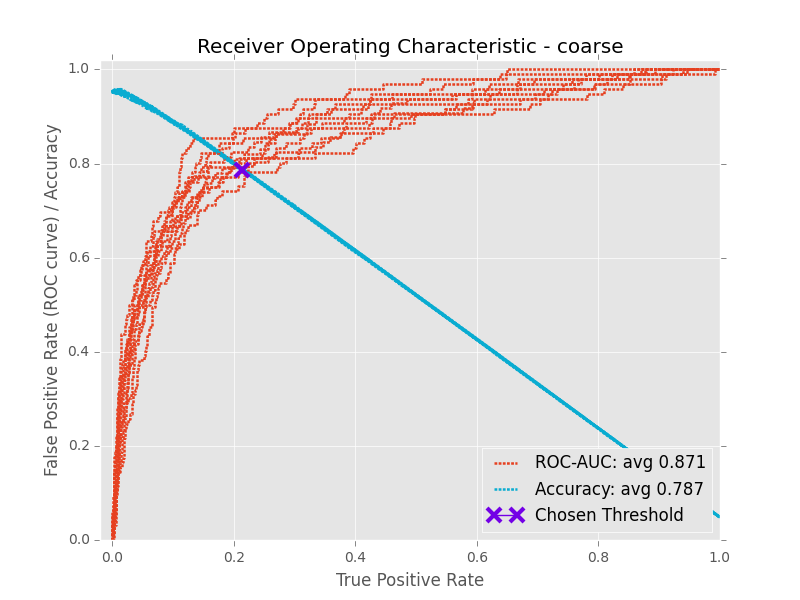
\includegraphics[width=\textwidth]{fig/LogReg_FindThreshold_RocCurve_coarse}
        \caption{Log Reg ROC Curves - coarse}
    \end{subfigure}%
    ~
    \begin{subfigure}[t]{0.5\textwidth}
        \centering
        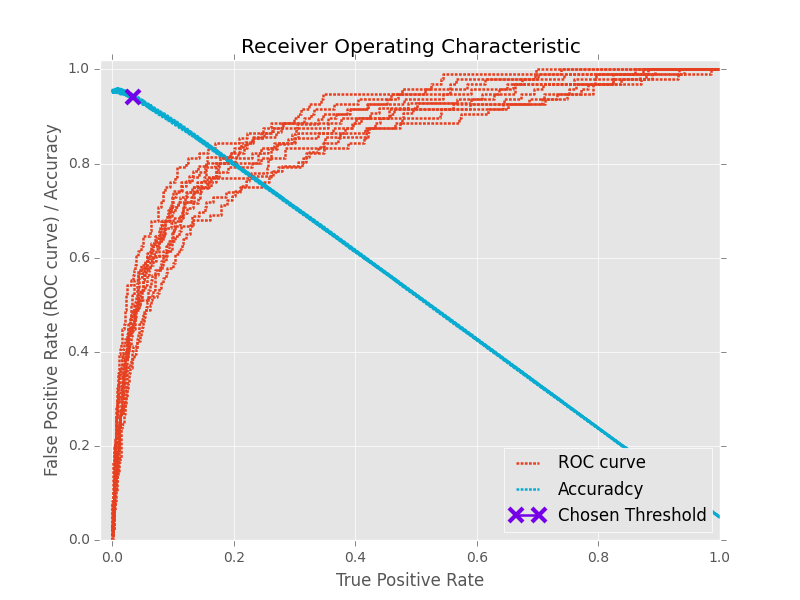
\includegraphics[width=\textwidth]{fig/LogReg_FindThreshold_RocCurve_fine}
        \caption{Log Reg ROC Curves - fine}
    \end{subfigure}
    \caption{Fine has a higher accuracy than coarse at the default threshold.}
\end{figure*}
\FloatBarrier


\FloatBarrier
\begin{figure*}[!htb]
    \centering
    \begin{subfigure}[t]{0.5\textwidth}
        \centering
        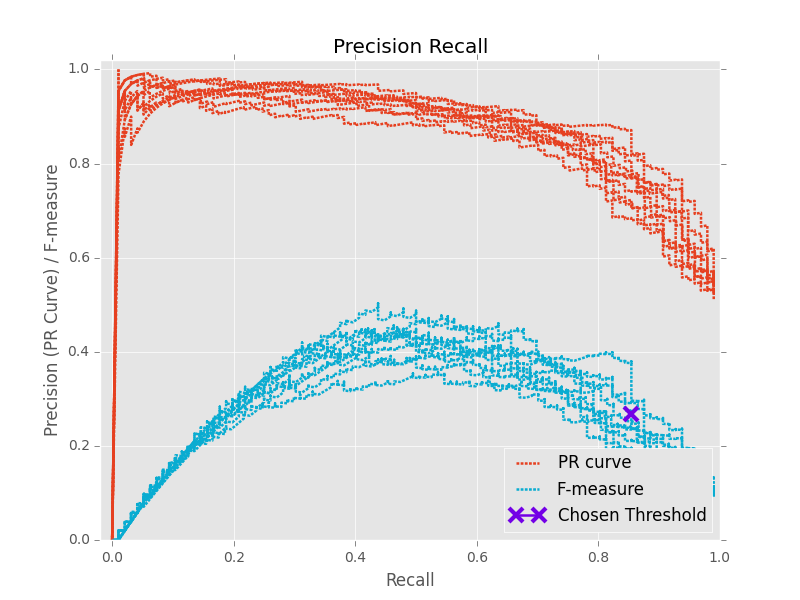
\includegraphics[width=\textwidth]{fig/LogReg_FindThreshold_PrCurve_coarse}
        \caption{Log Reg Pr Curves - coarse}
    \end{subfigure}%
    ~
    \begin{subfigure}[t]{0.5\textwidth}
        \centering
        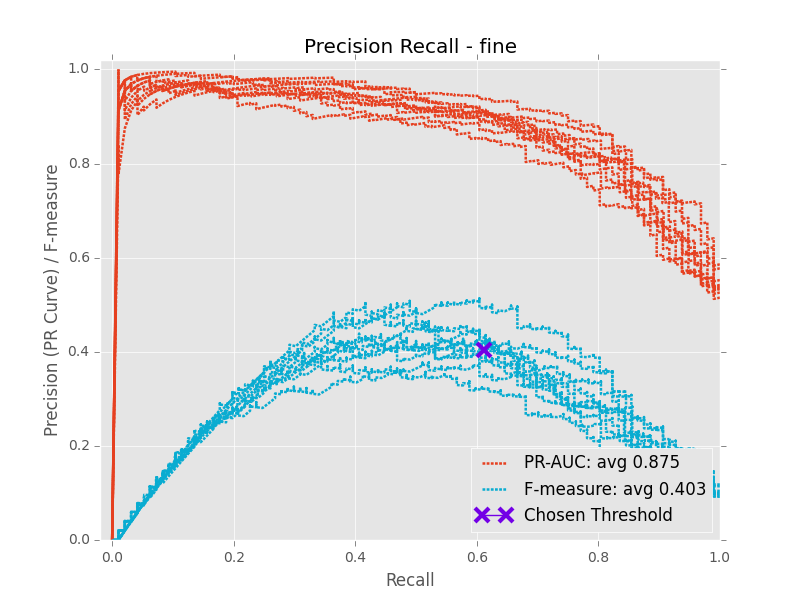
\includegraphics[width=\textwidth]{fig/LogReg_FindThreshold_PrCurve_fine}
        \caption{Log Reg Pr Curves - fine}
    \end{subfigure}
    \caption{The fine threshold occurs at a point on the pr-curve associated with a higher
    f-measure than the coarse curves.}
\end{figure*}
\FloatBarrier




\FloatBarrier
\begin{figure*}[!htb]
    \centering
    \begin{subfigure}[t]{0.5\textwidth}
        \centering
        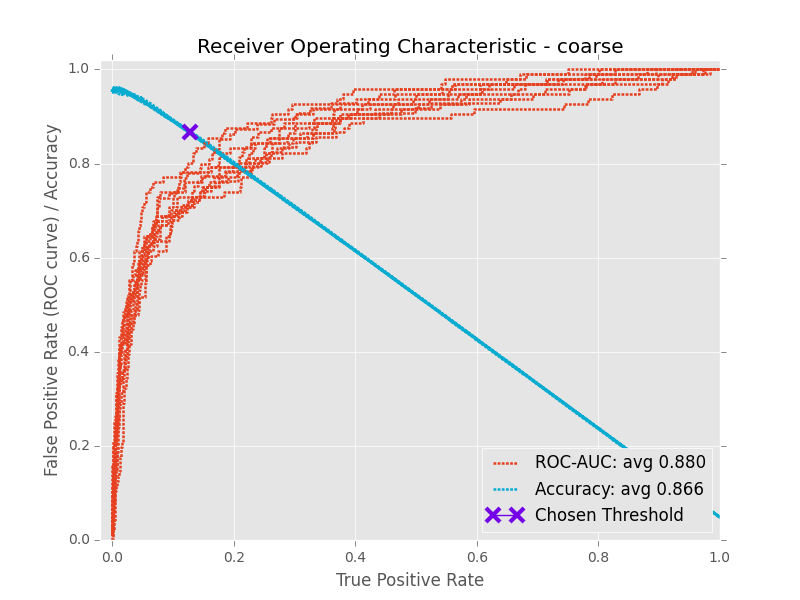
\includegraphics[width=\textwidth]{fig/SVM_FindThreshold_RocCurve_coarse}
        \caption{SVM ROC Curves - coarse}
    \end{subfigure}%
    ~
    \begin{subfigure}[t]{0.5\textwidth}
        \centering
        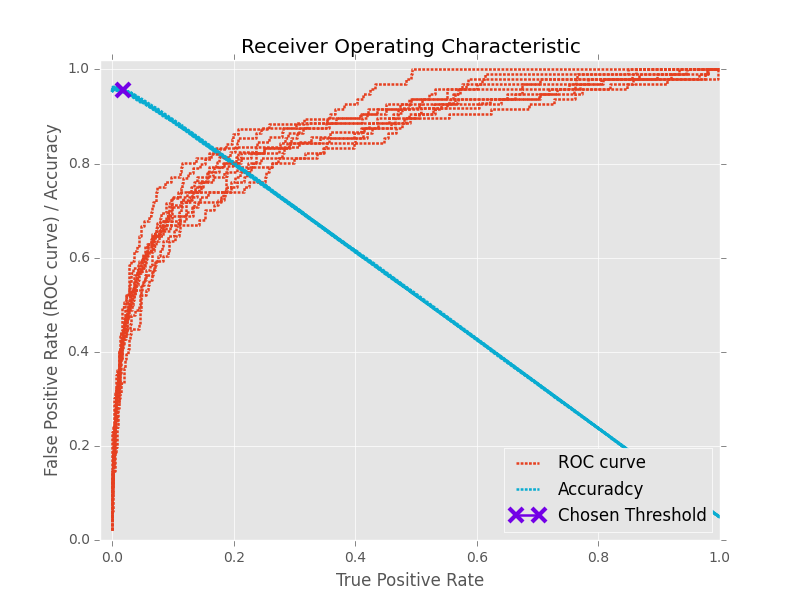
\includegraphics[width=\textwidth]{fig/SVM_FindThreshold_RocCurve_fine}
        \caption{SVM ROC Curves - fine}
    \end{subfigure}
    \caption{SVM results are similar between coarse and fine.}
\end{figure*}
\FloatBarrier


\FloatBarrier
\begin{figure*}[!htb]
    \centering
    \begin{subfigure}[t]{0.5\textwidth}
        \centering
        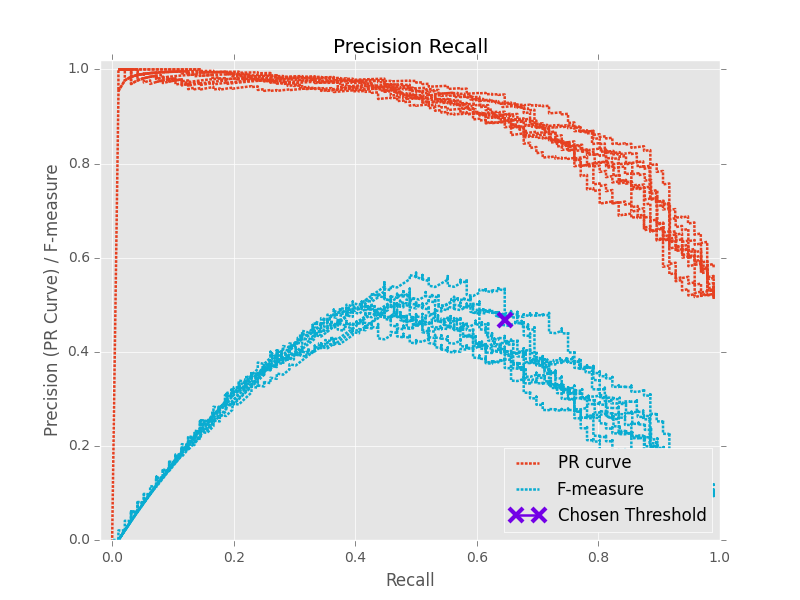
\includegraphics[width=\textwidth]{fig/SVM_FindThreshold_PrCurve_coarse}
        \caption{SVM Pr Curves - coarse}
    \end{subfigure}%
    ~
    \begin{subfigure}[t]{0.5\textwidth}
        \centering
        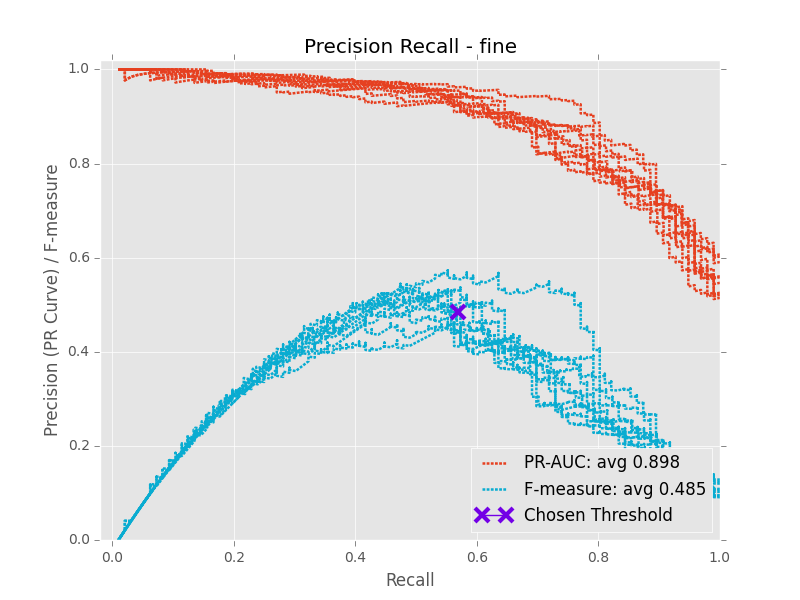
\includegraphics[width=\textwidth]{fig/SVM_FindThreshold_PrCurve_fine}
        \caption{SVM Pr Curves - fine}
    \end{subfigure}
    \caption{SVM results for PR-curves and F-measure have coarse and fine picking
    different parts of the curves for their respective thresholds, coarse f1 avg is
    slightly higher at 0.468 compared to 0.457 for fine.}
\end{figure*}
\FloatBarrier





\section{Active vs Passive curves}
\par The following plots were obtained with a round batch size of 100
and a starter set of 1040 instances out of the total 2098 instances.
The plots are the average of 10 folds, for each fold a test set of 2010
containing representatives of each class was held out, out of the remaining
18088, the starter set was selected which again contained representatives of
each class. Coarse and fine classifiers share the same starter set. During
 each round coarse and fine classifiers are trained on their corresponding
 sets, metrics are outputted on the held out test set, then confidence estimates
 are ran on the remaining eligible instances. Eligible instances are kept in
 separate sets for coarse and fine, 100 of the most uncertain instances are removed
 from each eligible set and added to its corresponding coarse or fine set to be
 trained on for the next round.


\FloatBarrier
\subsection{Plots for Logistic Regression Active vs Passive curves}
\begin{figure}[!htb]
	\centering
    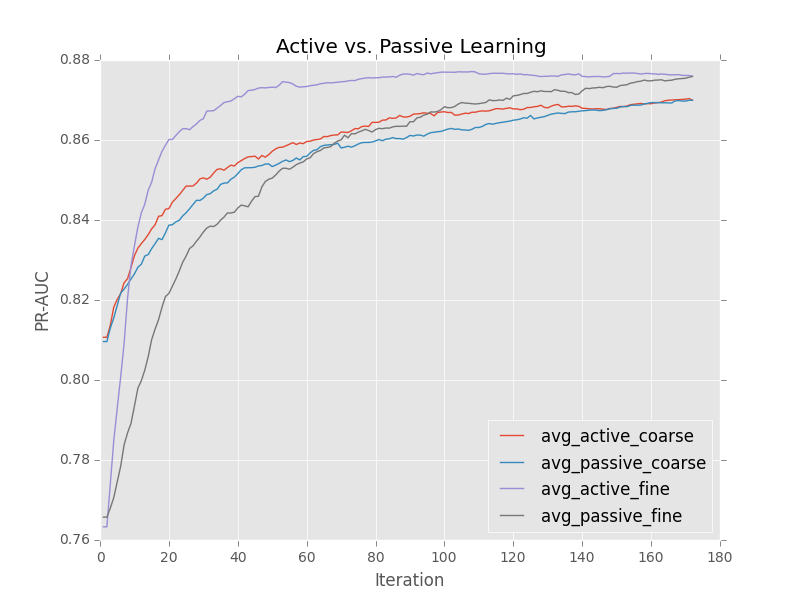
\includegraphics[width=1.0\columnwidth]{fig/ActiveVsPassivePRLR}
    \label{fig:ActiveVsPassivePRLR}
    \caption{The PR AUC curves for rounds with the Logistic
Regression classifier conforms to expectations, with active-fine having
the highest performance. Active-coarse outperforms passive-coarse. Passive-fine
doesn't outperform the coarse classifiers until rnd 100. }
\end{figure}
\FloatBarrier

\FloatBarrier
\begin{figure}[!htb]
	\centering
    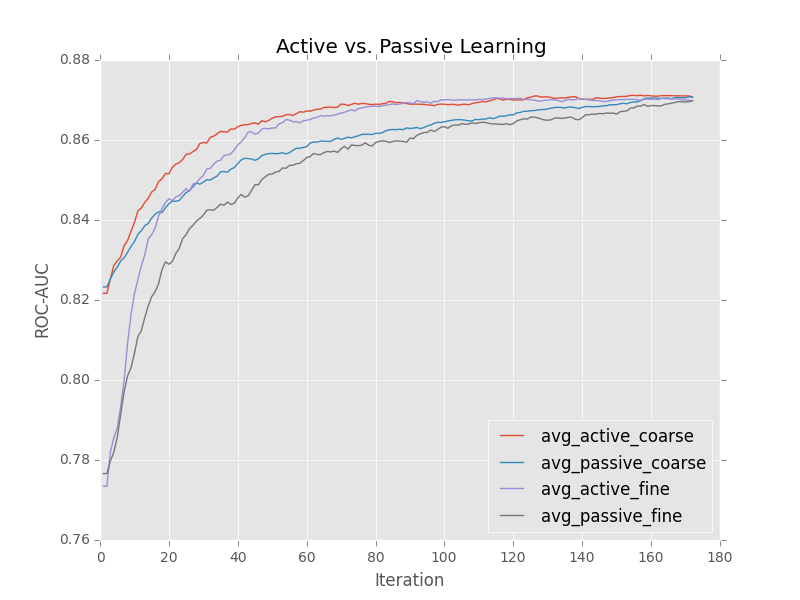
\includegraphics[width=1.0\columnwidth]{fig/ActiveVsPassiveROCLR}
    \label{fig:ActiveVsPassiveROCLR}
    \caption{The ROC AUC curves for rounds with the
Logistic Regression classifier. The active curves beat out the passive
curves for both coarse and fine. Coarse roc starts with an advantage over
fine as in the PR curves. Both converge to the same rate after roc auc level after 80.}
\end{figure}
\FloatBarrier

\FloatBarrier
\begin{figure}[!htb]
	\centering
    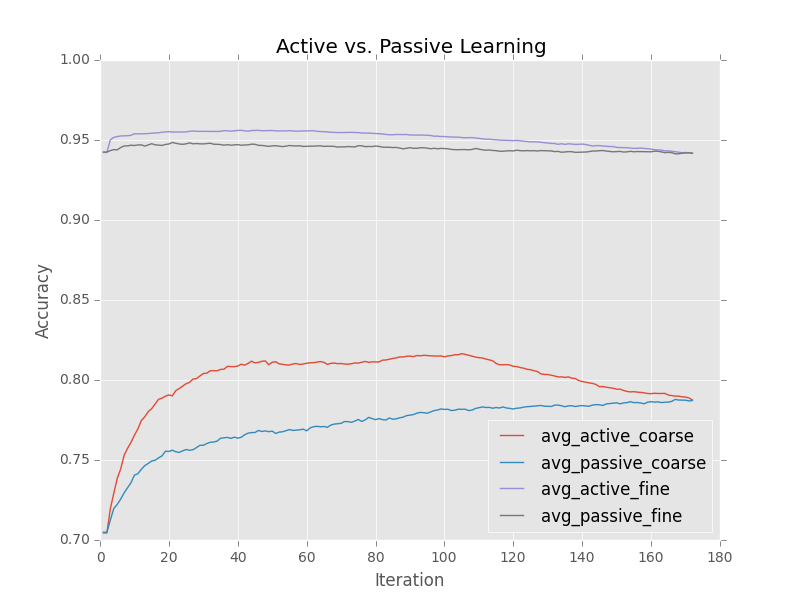
\includegraphics[width=1.0\columnwidth]{fig/ActiveVsPassiveAccLR}
    \label{fig:ActiveVsPassiveAccLR}
    \caption{The accuracy of the fine classifiers stays at
roughly the same rate throughout the rounds, this is due to an effective
weighting scheme for the fine grained classifiers. The active coarse accuracy
drops towards the end due to an increase in false positives as more negative
instances are added in the later rounds.}
\end{figure}
\FloatBarrier

\FloatBarrier
\begin{figure}[!htb]
	\centering
    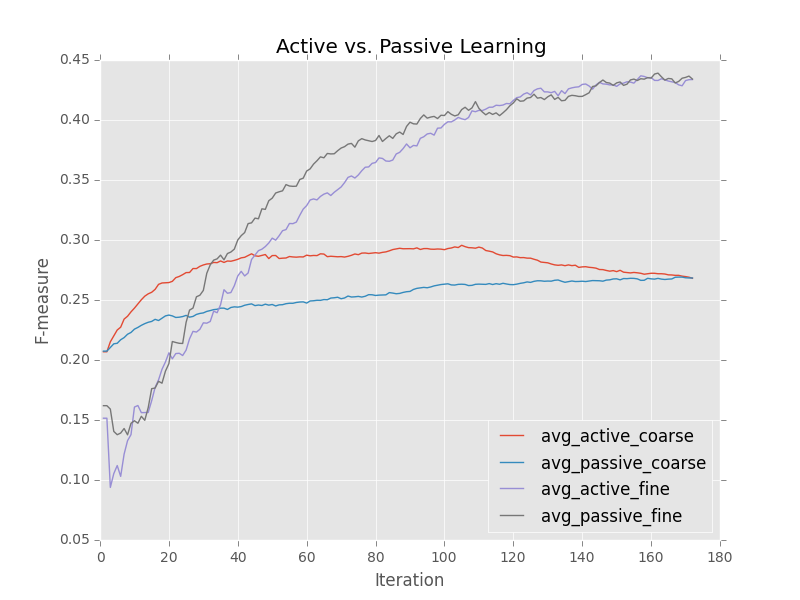
\includegraphics[width=1.0\columnwidth]{fig/ActiveVsPassiveF1LR}
    \label{fig:ActiveVsPassiveF1LR}
    \caption{The F-measure of the the fine classifiers increases
throughout the rounds as more true positives are predicted. The active coarse
again decreases at later rounds due to increased false positives.}
\end{figure}
\FloatBarrier









\FloatBarrier
\subsection{Plots for SVM Active vs Passive curves}
\begin{figure}[!htb]
	\centering
    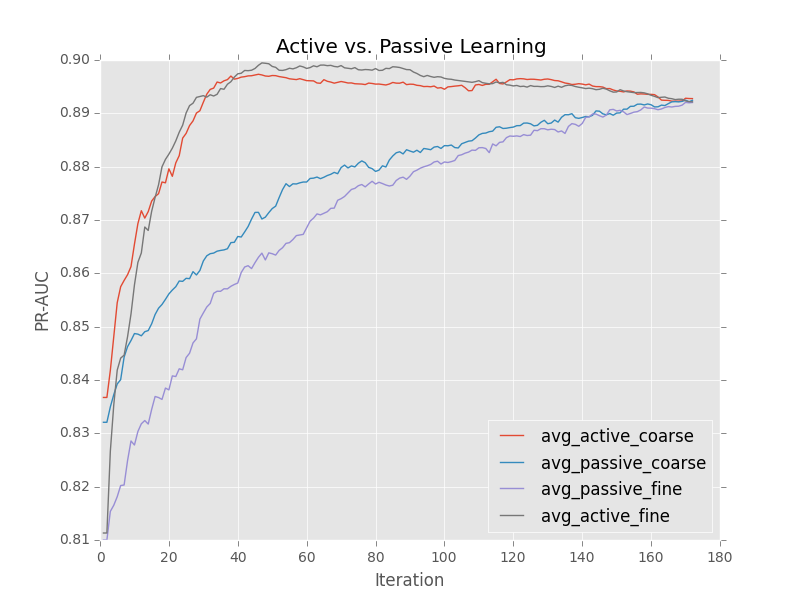
\includegraphics[width=1.0\columnwidth]{fig/ActiveVsPassivePRSVM}
    \label{fig:ActiveVsPassivePRSVM}
    \caption{The PR AUC curves for rounds with SVM show little
advantage for fine. The results are slightly different than the ones shown
on 2/14 due to fixing a bug with the code that wasn't performing the
preprocessing scaling for the SVM case at the same stage as it was being
done for the logistic regression classifier.}
\end{figure}
\FloatBarrier

\FloatBarrier
\begin{figure}[!htb]
	\centering
    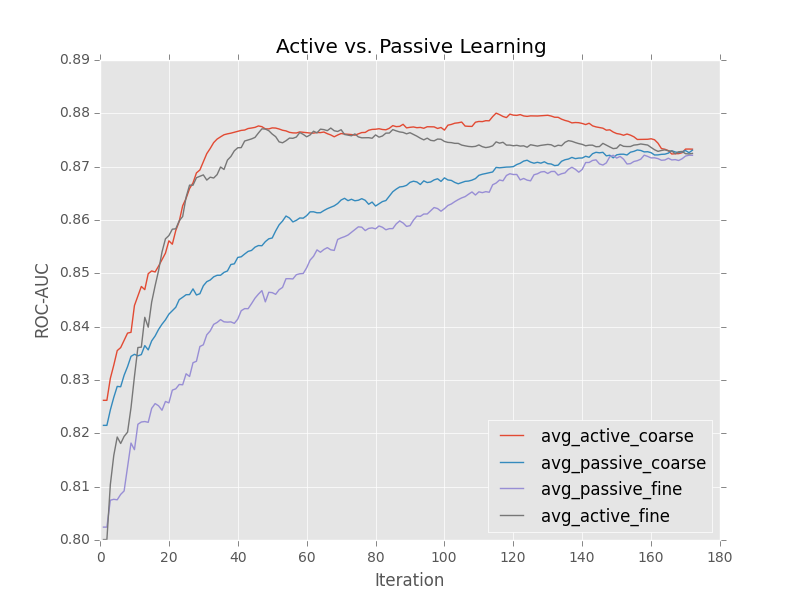
\includegraphics[width=1.0\columnwidth]{fig/ActiveVsPassiveROCSVM}
    \label{fig:ActiveVsPassiveROCSVM}
    \caption{The ROC curves show more of an advantage for coarse classifiers.}
\end{figure}
\FloatBarrier


\FloatBarrier
\begin{figure}[!htb]
	\centering
    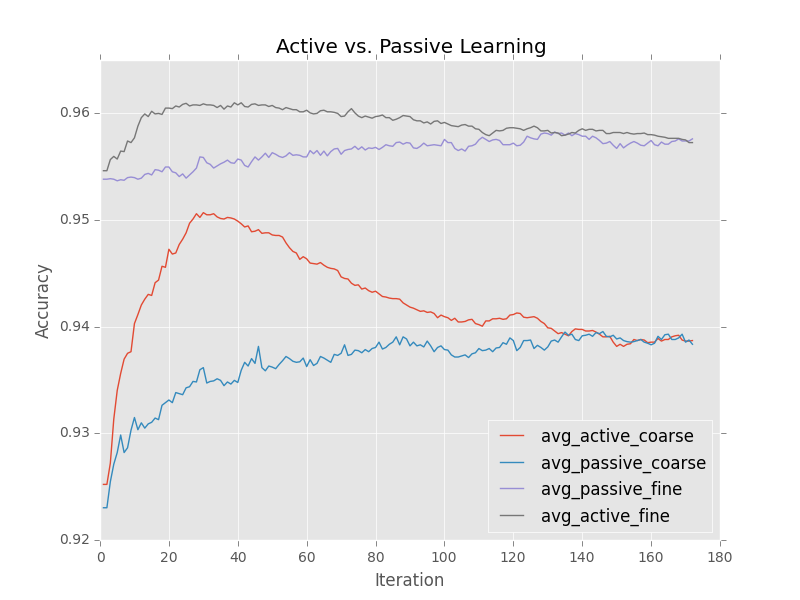
\includegraphics[width=1.0\columnwidth]{fig/ActiveVsPassiveAccSVM}
    \label{fig:ActiveVsPassiveAccSVM}
    \caption{The accuracy for the coarse decreases sharply due
to coarse predicting steadily more false positives, behaving similar to the
Log Reg case. Fine accuracy is higher due to predicting less false positives
than coarse. Fine also predicts less true positives, compare apx. 37 to apx.
60 t.p. for coarse at round 60.}
\end{figure}
\FloatBarrier

\FloatBarrier
\begin{figure}[!htb]
	\centering
    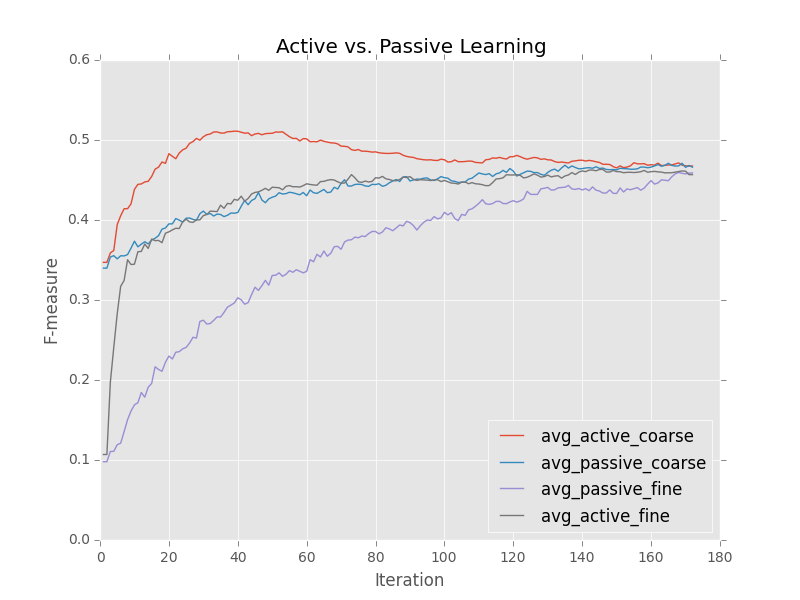
\includegraphics[width=1.0\columnwidth]{fig/ActiveVsPassiveF1SVM}
    \label{fig:ActiveVsPassiveF1SVM}
    \caption{The F-measure favors coarse, and trends to the same level
    for both coarse and fine.}
\end{figure}
\FloatBarrier


\break

\FloatBarrier
\section{Plots for FFR experiments}
\begin{figure}[!htb]
	\centering
    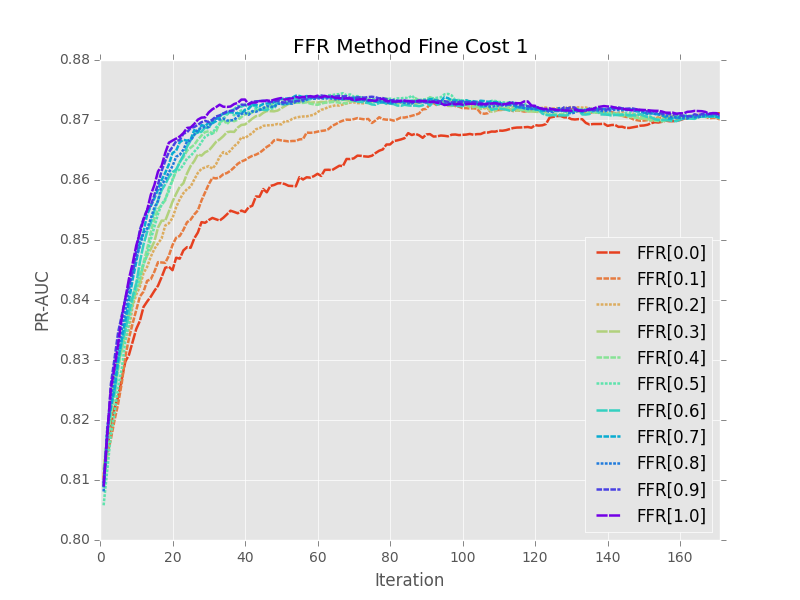
\includegraphics[width=1.0\columnwidth]{fig/FFR_PR_Cost1_rnds0_171}
    \label{fig:FFR_PR_Cost1}
    \caption{The strategy is changed from purchasing a set number of instances
    per round to having a set budget per round and spending a portion of that budget
    on fine and coarse grained labels. For this curve the fine and coarse grain labels
    both have a cost of 1. The purple 1.0 curve shows that if only fine grained labels
    are purchased, the highest performing PR-AUC can be obtained. The results are an
    average of 10 folds.}
\end{figure}
\FloatBarrier

\FloatBarrier
\begin{figure}[!htb]
	\centering
    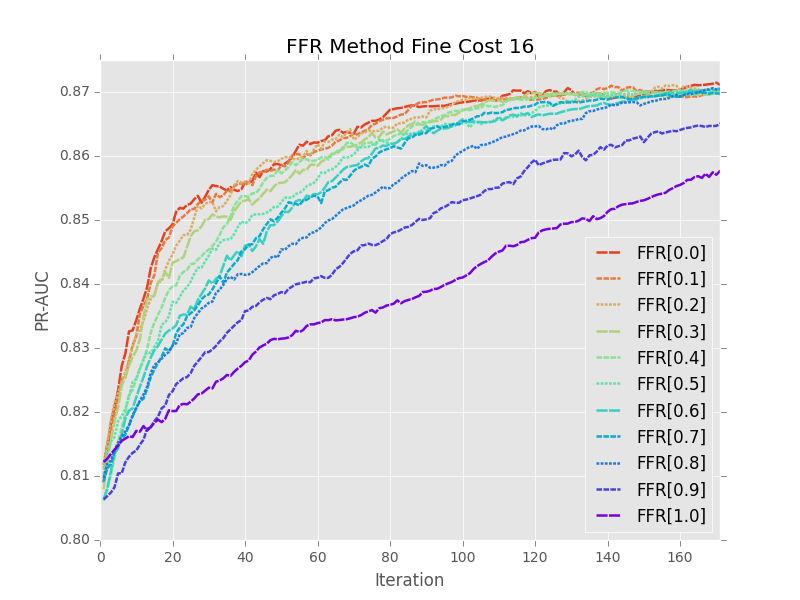
\includegraphics[width=1.0\columnwidth]{fig/FFR_PR_Cost16_rnds0_171}
    \label{fig:FFR_PR_Cost16_rnds0_171}
    \caption{The fine cost is increased to 16. The budget for each iteration is 100, and
    for the case of the 0.5 curve, 50 instances are bought for coarse and 3.125 instances are
    bought for fine. The remainder 0.125 is then turned into a 0.125 chance for any round to
    purchase an extra fine label. The round size for the FFR 1.0 curve is very small, with only
    7 labels purchased per iteration. The cost is to high for the fine label advantage to offset
    the decreased number of instances purchased.}
\end{figure}
\FloatBarrier


\FloatBarrier
\begin{figure}[!htb]
	\centering
    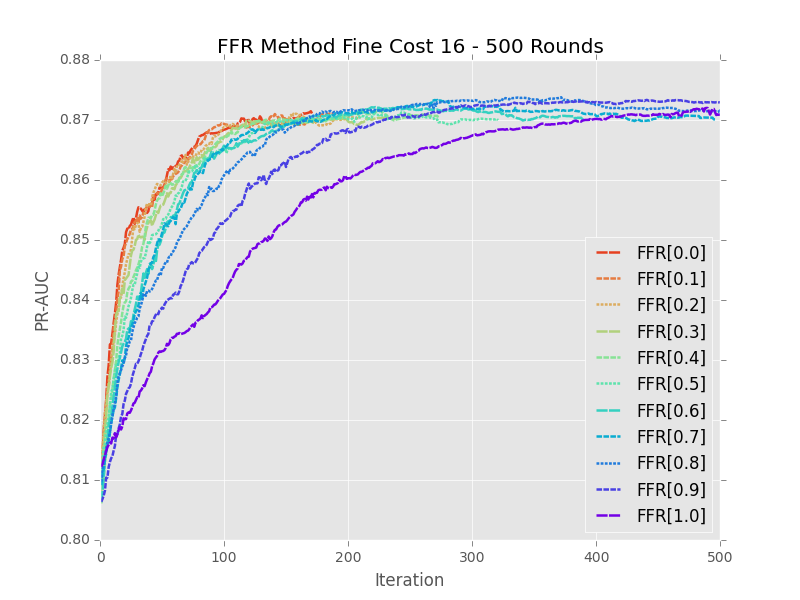
\includegraphics[width=1.0\columnwidth]{fig/FFR_PR_Cost16_rnds0_500}
    \label{fig:FFR_PR_Cost16_rnds0_500}
    \caption{This shows the iterations continuing through round 500, the curves
    with the higher fine rates eventually settle to the same end point that the
    curves with the high rates of coarse labels purchased achieved at previous
    iterations.}
\end{figure}
\FloatBarrier



\FloatBarrier
\begin{figure}[!htb]
	\centering
    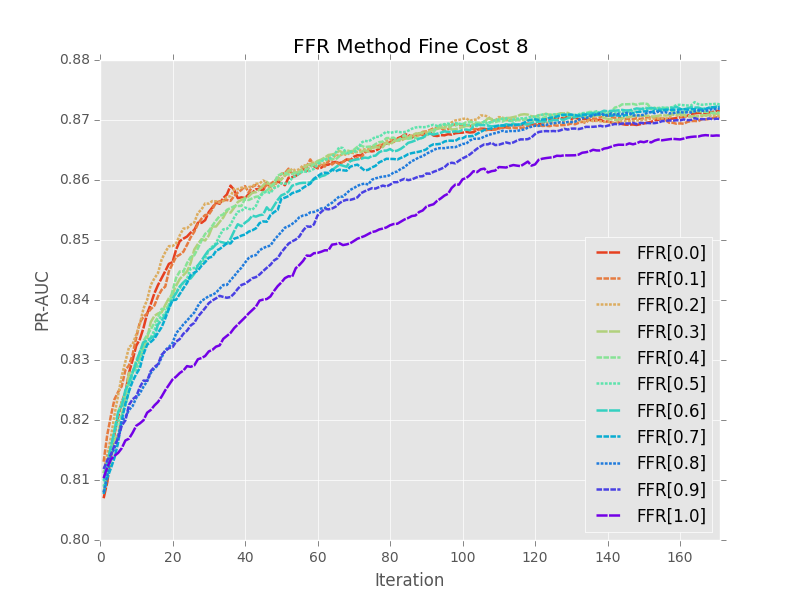
\includegraphics[width=1.0\columnwidth]{fig/FFR_PR_Cost8_rnds0_171}
    \label{fig:FFR_PR_Cost8_rnds0_171}
    \caption{At fine cost 8 the FFR 0.0 rate is no longer the best option, 0.1
    generally outperforms 0.0 slightly.}
\end{figure}
\FloatBarrier


\FloatBarrier
\begin{figure}[!htb]
	\centering
    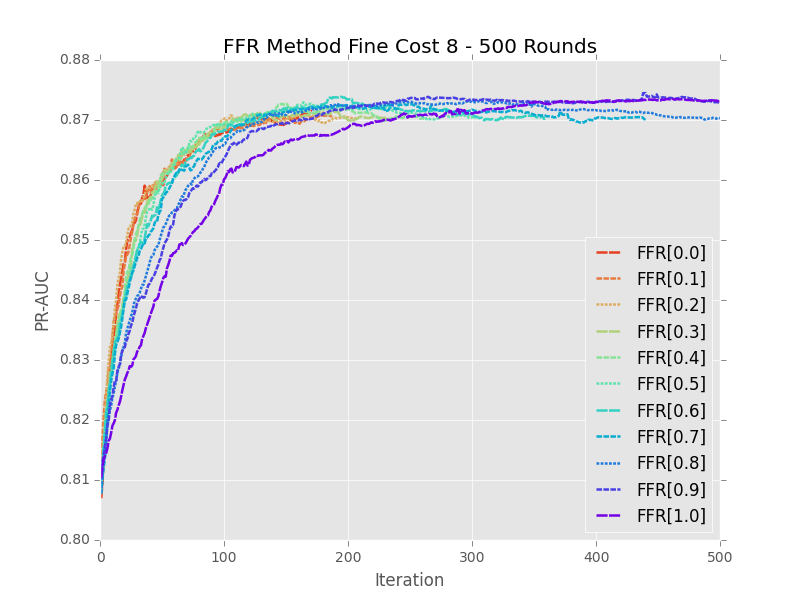
\includegraphics[width=1.0\columnwidth]{fig/FFR_PR_Cost8_rnds0_500}
    \label{fig:FFR_PR_Cost8_rnds0_500}
    \caption{The extended picture of the FFR cost 8. The round size for FFR 1.0
    is small, only 13 instances purchase per iteration.}
\end{figure}
\FloatBarrier


\FloatBarrier
\begin{figure}[!htb]
	\centering
    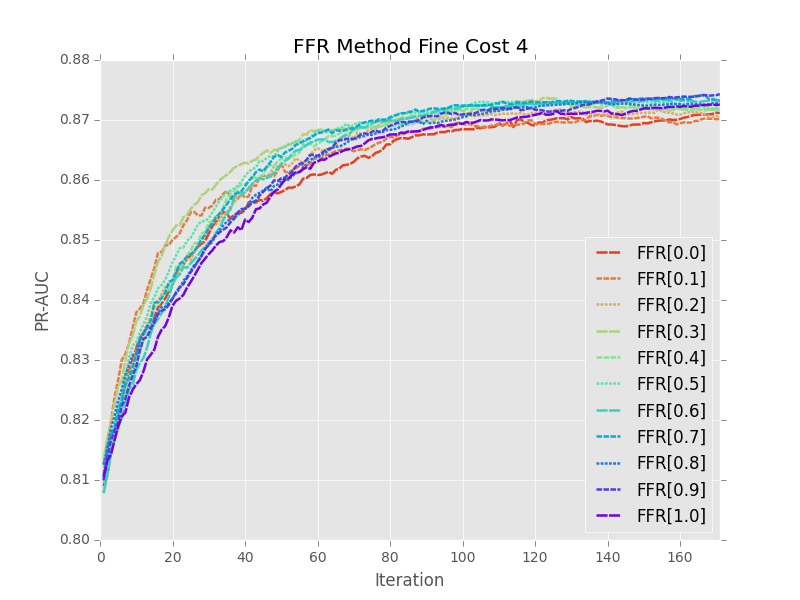
\includegraphics[width=1.0\columnwidth]{fig/FFR_PR_Cost4_rnds0_171}
    \label{fig:FFR_PR_Cost4_rnds0_171}
    \caption{At fine cost 4, FFR 0.3 appears to be the highest performing rate.}
\end{figure}
\FloatBarrier


\FloatBarrier
\begin{figure}[!htb]
	\centering
    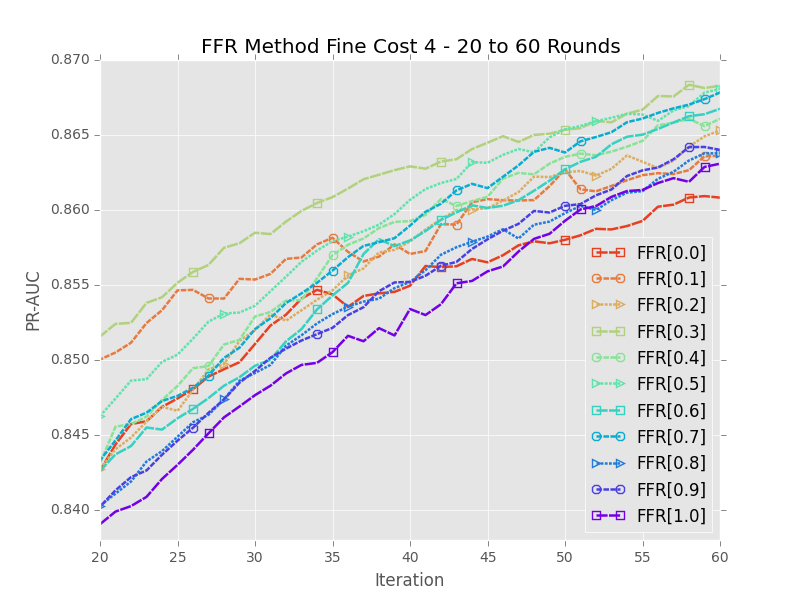
\includegraphics[width=1.0\columnwidth]{fig/FFR_PR_Cost4_rnds20_60}
    \label{fig:FFR_PR_Cost4_rnds20_60}
    \caption{The fine cost 4 curves shown expanding the rounds 20-60.}
\end{figure}
\FloatBarrier


\FloatBarrier
\begin{figure}[!htb]
	\centering
    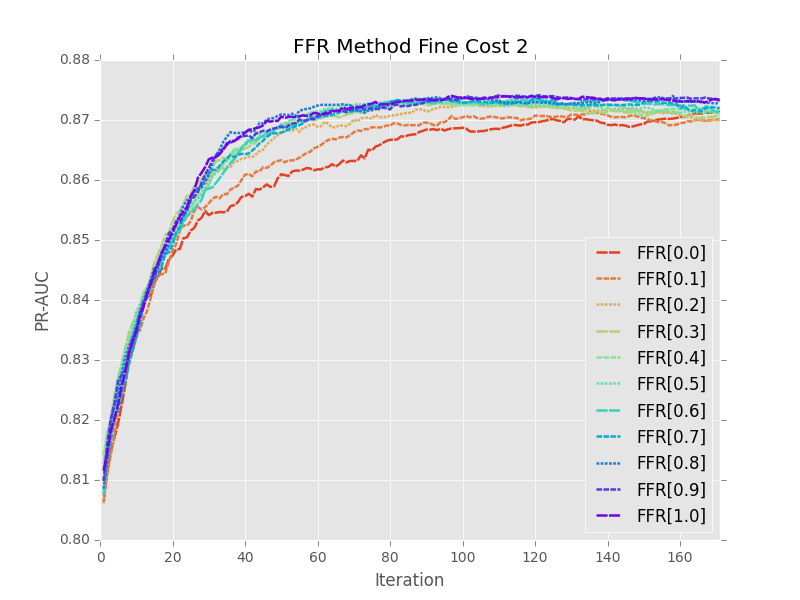
\includegraphics[width=1.0\columnwidth]{fig/FFR_PR_Cost2_rnds0_171}
    \label{fig:FFR_PR_Cost2_rnds0_171}
    \caption{At fine cost 2, the preferred rate jumps up to 0.8,
    similar to the cost 1 results.}
\end{figure}
\FloatBarrier

\FloatBarrier
\begin{figure}[!htb]
	\centering
    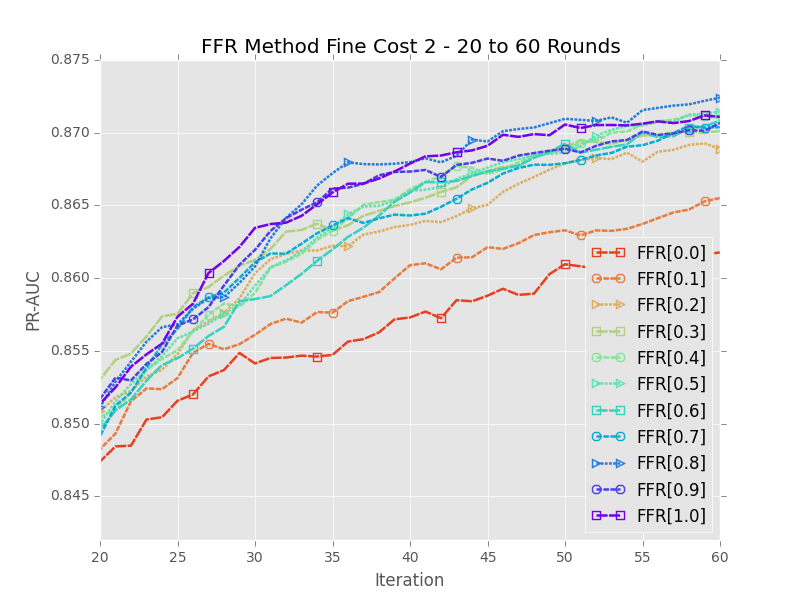
\includegraphics[width=1.0\columnwidth]{fig/FFR_PR_Cost2_rnds20_60}
    \label{fig:FFR_PR_Cost2_rnds20_60}
    \caption{The fine cost 2 curves shown expanding rounds 20-60.}
\end{figure}
\FloatBarrier



\chapter{Conclusions and Future Work}\label{chap:math}
\par I should probably do the Bandit experiments.










%% backmatter is needed at the end of the main body of your thesis to
%% set up page numbering correctly for the remainder of the thesis
\backmatter

%% Start the correct formatting for the appendices
\appendix

\chapter{Tuning the fine grained classes}
\par All the data and results for tuning the fine grained classes.

%% Bibliography goes here (You better have one)
%% BibTeX is your friend
%\bibliographystyle{plain}
\bibliographystyle{IEEEtran}
\bibliography{IEEEabrv,nuthesis}
%% Pull in all the entries in the bibtex file. Is is a useful trick to
%% check all your references.
\nocite{*}


%% Index go here (if you have one)

\end{document}
\endinput
%%
%% End of file `thesis-test.tex'.
